%% 
%% Copyright 2019-2024 Elsevier Ltd
%% 
%% This file is part of the 'CAS Bundle'.
%% --------------------------------------
%% 
%% It may be distributed under the conditions of the LaTeX Project Public
%% License, either version 1.3c of this license or (at your option) any
%% later version.  The latest version of this license is in
%%    http://www.latex-project.org/lppl.txt
%% and version 1.3c or later is part of all distributions of LaTeX
%% version 1999/12/01 or later.
%% 
%% The list of all files belonging to the 'CAS Bundle' is
%% given in the file `manifest.txt'.
%% 
%% Template article for cas-dc documentclass for 
%% double column output.

\documentclass[a4paper,fleqn]{cas-dc}

% If the frontmatter runs over more than one page
% use the longmktitle option.

%\documentclass[a4paper,fleqn,longmktitle]{cas-dc}

\usepackage[numbers]{natbib}
%\usepackage[authoryear]{natbib}
\usepackage{url}
\usepackage{algorithm}
\usepackage{algorithmic}
\usepackage{adjustbox} % shrink-only table scaling; keeps a uniform table font size (see Sec. tables)
\usepackage{subcaption}

% Transitional guard for the removed line-numbering build.
% lineno.sty wrote ~1,400 \@LN{<line>}{<col>} entries into the .aux file.
% Overleaf reuses its cached .aux across compiles, so the first build after
% lineno was dropped reads those entries with \@LN no longer defined and
% aborts with "Undefined control sequence". Absorbing them here lets that
% build finish, after which the .aux is rewritten without them.
% Safe to delete once the project has compiled cleanly.
\makeatletter
\providecommand{\@LN}[2]{}
\makeatother

% --- Float placement -------------------------------------------------------
% The cas-dc class redefines the figure environment so that its optional
% argument is a key-value list, not a LaTeX placement specifier: [!t] is read
% as the CAS key "pos" and every standard float parameter is ignored. Figures
% must therefore be positioned with pos=..., and each one below uses
% pos=htbp so it can settle in the column where it is cited. Without this the
% figures were deferred behind the 14 tables of Section 4 and printed after
% the bibliography. pos=H is deliberately avoided: it forbids text flowing
% past the float, which left large blanks at the foot of a column whenever a
% figure did not fit in the space remaining. Tables place correctly on their
% own and are left as they are.

%%%Author macros
\def\tsc#1{\csdef{#1}{\textsc{\lowercase{#1}}\xspace}}
\tsc{WGM}
\tsc{QE}
%%%

% Uncomment and use as if needed
%\newtheorem{theorem}{Theorem}
%\newtheorem{lemma}[theorem]{Lemma}
%\newdefinition{rmk}{Remark}
%\newproof{pf}{Proof}
%\newproof{pot}{Proof of Theorem \ref{thm}}

\begin{document}
\let\WriteBookmarks\relax
\def\floatpagepagefraction{1}
\def\textpagefraction{.001}

% Short title
\shorttitle{Protocol-Agnostic Intrusion Detection for Automotive Ethernet}

% Short author
\shortauthors{Y.~Kang et~al.}

% Main title of the paper
\title[mode = title]{Time-Aware Dual-Stream Masked Autoencoder for Protocol-Agnostic Intrusion Detection in Automotive Ethernet}

% First author
\author[1]{Yeonjae Kang}[orcid=0000-0003-0612-7638]
\ead{kangyj1995@korea.ac.kr}
\credit{Conceptualization, Methodology, Software, Validation, Formal analysis, Investigation, Data curation, Visualization, Writing -- original draft}

\author[1]{Huy Kang Kim}[orcid=0000-0002-0760-8807]
\ead{cenda@korea.ac.kr}
\credit{Resources, Supervision, Writing -- review \& editing}

\author[2]{Seonghoon Jeong}[orcid=0000-0001-5638-2851]
\cormark[1]
\ead{seonghoon@sookmyung.ac.kr}
\credit{Conceptualization, Methodology, Supervision, Project administration, Writing -- review \& editing}

% Address/affiliation
\affiliation[1]{organization={School of Cybersecurity, Korea University},
            addressline={145 Anam-ro, Seongbuk-gu},
            city={Seoul},
            postcode={02841},
            country={Republic of Korea}}

\affiliation[2]{organization={Division of Artificial Intelligence Engineering, Sookmyung Women's University},
            addressline={100 Cheongpa-ro 47-gil, Yongsan-gu},
            city={Seoul},
            postcode={04310},
            country={Republic of Korea}}

% Corresponding author text
\cortext[1]{Corresponding author.}

% Here goes the abstract
\begin{abstract}
Automotive Ethernet (AE) is becoming the primary in-vehicle communication backbone for bandwidth-intensive applications such as camera streaming and ADAS, yet its security remains underexplored. Existing in-vehicle IDS predominantly rely on supervised learning or protocol-specific parsing, requiring labeled attack data and domain expertise difficult to obtain in real deployments.

We propose a protocol-agnostic, unsupervised IDS based on a dual-stream masked autoencoder trained exclusively on unlabeled normal traffic. The model processes 64-packet windows through a Transformer encoder over raw byte content and a residual 1D-CNN over inter-packet byte differences, fused via a delta-conditioned gated residual mechanism into a latent representation through attention pooling. Rather than the conventional sinusoidal scheme, the Transformer's positional encoding is conditioned on inter-packet capture timestamps, allowing it to jointly reason about content and arrival timing without protocol-specific parsing. Training uses packet-level masked reconstruction with a learnable mask token; at inference, anomalies are flagged by thresholding reconstruction error against the normal validation error distribution.

We evaluate on CarDS, a recently released real-vehicle AE dataset, using over 5.4 million normal packets for training and 27 attack files spanning 23 attack types, including network scanning, IP/MAC spoofing, and RTP stream injection. The proposed method achieves an F1-score of 0.9802, AUROC of 0.9976, and AUPRC of 0.9974, with near-perfect detection on scanning attacks (F1 up to 0.9993) and competitive performance on payload-substitution attacks. Ablation studies confirm that both the dual-stream design and time-aware encoding independently improve detection, with the latter substantially widening the threshold range over which performance remains stable.
\end{abstract}

% Use if graphical abstract is present
%\begin{graphicalabstract}
%\includegraphics{}
%\end{graphicalabstract}

% Research highlights
\begin{highlights}
\item Transformer and CNN streams jointly model packet bytes and inter-packet deltas
\item Trained only on normal traffic with no attack labels or protocol-specific parsing
\item Time-aware positional encoding from packet timing widens the stable threshold range
\item Achieves F1 0.9808 and AUROC 0.9974 across 27 real-vehicle attack captures
\item Presents the first anomaly detection study on the real-vehicle CarDS dataset
\end{highlights}


%\nocite{*}

% Keywords
% Each keyword is seperated by \sep
\begin{keywords}
Anomaly detection \sep Automotive Ethernet \sep In-vehicle network \sep Intrusion detection system \sep Masked autoencoder \sep Self-supervised learning
\end{keywords}

\maketitle
% Main text
\section{Introduction}
The rapid evolution of automotive architectures has driven a transition from traditional Controller Area Network (CAN) buses to high-speed Automotive Ethernet (AE), enabling bandwidth-intensive applications such as surround-view camera systems, LiDAR data transmission, and over-the-air (OTA) software updates~\cite{matheus2021automotive}. While this architectural shift brings substantial functional advantages, it simultaneously expands the attack surface of in-vehicle networks by exposing vehicles to a broader class of cyber threats previously associated with enterprise and industrial networks, including port scanning, address spoofing, and payload injection~\cite{douss2023state}.

Intrusion detection systems (IDS) have emerged as a primary defense mechanism for in-vehicle networks, and a substantial body of research has been devoted to CAN-based IDS leveraging statistical anomaly detection, machine learning, and deep learning approaches~\cite{lokman2019intrusion}. However, Automotive Ethernet presents fundamentally different traffic characteristics: packets carry variable-length raw byte payloads, traffic is heterogeneous across network segments (e.g., control traffic versus high-bandwidth RTP camera streams), and the protocol stack closely mirrors standard IP networking. These properties render CAN-specific detection methods inapplicable and necessitate purpose-built approaches for Automotive Ethernet.

A central challenge in developing IDS for automotive systems is the scarcity of labeled attack data. Collecting representative attack traffic in real vehicles is operationally constrained, and manually annotating large-scale packet captures is prohibitively expensive. As a result, supervised learning approaches -- which have achieved strong performance in controlled benchmark settings -- are difficult to deploy in practice, as they require comprehensive coverage of attack types at training time and fail to generalize to unseen attack variants~\cite{hindy2020taxonomy}. This motivates an unsupervised formulation of the intrusion detection problem, in which a model is trained exclusively on normal traffic and anomalies are identified as deviations from the learned normal behavior.

Self-supervised learning (SSL) has recently demonstrated remarkable success in learning rich representations from unlabeled data across vision~\cite{he2022masked}, language~\cite{devlin2019bert}, and time-series domains~\cite{yue2022ts2vec}. In particular, masked autoencoding -- wherein a model is trained to reconstruct randomly masked portions of its input -- has proven effective at capturing the underlying generative structure of complex sequential data. This property is well-suited to network traffic anomaly detection: a model that faithfully reconstructs normal packet sequences will produce elevated reconstruction errors when presented with anomalous traffic that deviates from learned patterns.

However, applying masked autoencoding to Automotive Ethernet traffic is non-trivial. Network packets contain two complementary sources of information that exhibit distinct statistical properties: the raw byte content of each packet, which encodes payload structure and protocol fields, and the inter-packet byte differences across a traffic sequence, which capture how each byte position evolves over consecutive packets. Modeling these two information sources with a single homogeneous encoder risks underutilizing either the global sequential structure or the per-byte temporal variation patterns. Furthermore, Automotive Ethernet carries heterogeneous traffic types within the same network, including low-bandwidth control packets and high-bandwidth RTP camera streams, each exhibiting distinct normal behavior and susceptibility to different attack classes.

To address these challenges, we propose a self-supervised dual-stream masked autoencoder for unsupervised intrusion detection in Automotive Ethernet networks. Given a sliding window of 64 consecutive packets, two specialized encoders are trained jointly to exploit the two complementary information sources described above. Global inter-packet structure is captured by a Transformer encoder operating on normalized raw byte content; critically, its positional encoding departs from the fixed sinusoidal scheme common to Transformer architectures and is instead conditioned on the actual inter-packet interval measured at capture time, so that the model reasons about \emph{when} a packet arrived rather than merely its rank within the window, without requiring any upper-layer protocol parsing. Complementing this global view, a residual 1D-CNN treats each byte position as an independent channel and convolves along the packet axis to track fine-grained, per-byte variation across consecutive packets -- variation that a window-wide attention mechanism is comparatively less suited to localize. The two streams are combined through a delta-conditioned gated residual mechanism, in which the CNN stream's own magnitude determines how strongly it corrects the Transformer representation; the fused sequence is then pooled via attention into a single latent vector, from which a conditioned decoder reconstructs the original packet content (Figure~\ref{fig:architecture}). The entire model is trained on normal traffic alone under a masked reconstruction objective with asymmetric loss weighting toward masked positions, and at inference an anomaly is flagged whenever the mean reconstruction error of a window exceeds a threshold calibrated on the normal traffic error distribution.

We evaluate the proposed method on CarDS~\cite{hellemans2025cards}, to our knowledge the first publicly available real-vehicle Automotive Ethernet capture encompassing both control-network and RTP camera-stream traffic across multiple driving scenarios, with attack coverage spanning Nmap-based scanning, IP/MAC address spoofing, and RTP stream replacement. Despite using no attack labels during training, the proposed method reaches an overall F1-score of 0.9808 (AUROC 0.9974, AUPRC 0.9972) across 27 attack files and 23 attack configurations -- performance that, as detailed in Section~\ref{sec:baseline}, closely tracks a fully supervised baseline trained with complete attack labels. Detection is near-perfect on scanning and spoofing attacks (F1 up to 0.9993) and remains competitive on the structurally harder RTP stream replacement category (F1 up to 0.9217), where the attack alters only payload content while leaving packet timing and header structure intact. The architectural ablations reported in Section~\ref{sec:ablation} isolate the source of this performance: both the dual-stream design and the time-aware positional encoding contribute independently, with the latter also markedly extending the range of detection thresholds over which performance stays stable -- an important property for practical deployment (Section~\ref{sec:discussion}).

The main contributions of this paper are as follows:
\begin{itemize}
\item To our knowledge, we present the first anomaly detection study conducted on the CarDS Automotive Ethernet dataset, establishing evaluation protocols and performance baselines for this newly available real-vehicle benchmark.

\item We propose a protocol-agnostic (i.e., parsing-free) dual-stream masked autoencoder for unsupervised Automotive Ethernet intrusion detection: a Transformer encoder over raw packet content, conditioned on a time-aware positional encoding derived from real inter-packet capture timing rather than fixed sequence rank, combined with a residual CNN encoder over inter-packet byte differences through a delta-conditioned gated residual fusion mechanism. The model is trained via packet-level masked reconstruction on unlabeled normal traffic alone, requiring no protocol-specific parsing or labeled attack data. Ablation studies confirm that both the dual-stream design and the time-aware encoding independently improve detection, with the latter also substantially widening the range of thresholds over which performance remains stable.

\item We conduct extensive experiments against representative existing approaches and ablation studies across 27 real-vehicle attack files spanning 23 attack configurations, providing detailed analysis of detection performance across heterogeneous attack categories.
\end{itemize}

The remainder of this paper is organized as follows. Section~\ref{sec:relatedwork} reviews related work on in-vehicle network intrusion detection and self-supervised learning for anomaly detection. Section~\ref{sec:methodology} describes the proposed method in detail. Section~\ref{sec:experiments} presents the experimental setup, results, and ablation studies. Section~\ref{sec:discussion} discusses the broader implications of these results, including the comparison with baseline methods, the role of RTP-specific behavior, and practical deployment considerations. Section~\ref{sec:conclusion} concludes the paper and outlines directions for future work.
\section{Related Work}
\label{sec:relatedwork}
\subsection{Intrusion Detection Systems for In-Vehicle Networks}
Early research on in-vehicle network security focused predominantly on the Controller Area Network (CAN) protocol, which has been the dominant communication standard in automotive systems for decades. A wide range of IDS approaches have been proposed for CAN: rule-based methods that flag violations of message periodicity and identifier frequency~\cite{song2016intrusion}, statistical approaches based on entropy~\cite{muter2011entropy}, and machine learning methods spanning support vector machines~\cite{bari2023intrusion}, random forests~\cite{caivano2024marea}, recurrent neural networks~\cite{taylor2016anomaly}, and deep neural networks~\cite{kang2016intrusion}. Survey studies have systematically categorized these approaches and identified key limitations, including the substantial re-engineering required to port a given detection scheme to a different vehicle make or model, since CAN message implementations and specifications are largely vehicle-specific~\cite{sharmin2024benchmarking, lampe2023survey}.

With the adoption of Automotive Ethernet as the backbone for high-bandwidth in-vehicle communication, attention has begun to shift toward Ethernet-specific security. Several studies have examined vulnerability analysis and attack modeling for Automotive Ethernet~\cite{de2024systematic, fotouhi2023assessing}, and initial IDS proposals have framed intrusion detection as a traffic classification problem, relying on packet-level features extracted directly from payloads~\cite{jeong2021convolutional}, packet byte features homogenized to a fixed length and reduced by feature selection~\cite{shibly2023feature}, or protocol-specific header fields processed by a sequential classifier~\cite{alkhatib2021some}. However, the majority of existing Automotive Ethernet IDS proposals rely on supervised learning, requiring labeled examples of each attack type during training~\cite{jeong2021convolutional,alkhatib2021some}. This dependency is problematic in practice, as the space of possible attacks against Automotive Ethernet is large and continuously evolving, making comprehensive labeled dataset collection infeasible. In contrast, our method requires no labeled attack data, learning exclusively from normal traffic and detecting anomalies as deviations from the learned normal behavior.

Table~\ref{tab:relatedwork_ae} summarizes these Automotive Ethernet IDS approaches alongside the proposed method. The proposed method is the only one of the compared approaches that is simultaneously label-free in training and protocol-agnostic: AERO removes the labeling requirement but still depends on protocol-informed feature engineering, while the supervised and semi-supervised approaches depend on both labels and protocol-specific representations. Labels re-enter only when the detection threshold is selected, which applies to the proposed method as well (Section~\ref{sec:limitations}).

\begin{table*}[!tbp]
\centering
\caption{Qualitative comparison of existing Automotive Ethernet IDS approaches. Label Req.: fraction of labeled attack data required for training.}
\label{tab:relatedwork_ae}
\footnotesize
\begin{tabular}{lcccc}
\toprule
\textbf{Method} & \textbf{Paradigm} & \textbf{Label Req.} & \textbf{Feature} & \textbf{Protocol-Agnostic} \\
\midrule
Jeong et al.~\cite{jeong2021convolutional} & Supervised & 100\% & Protocol-specific (AVTP payload) & No \\
Alkhatib et al.~\cite{alkhatib2021some} & Supervised & 100\% & Protocol-specific (SOME/IP header fields) & No \\
Shibly et al.~\cite{shibly2023feature} & Semi-supervised & $\sim$10\% & Padded packet bytes + feature selection & No \\
AERO~\cite{jeong2023aero} & Unsupervised & 0\% & Engineered, protocol-informed (multimodal) & No \\
\textbf{Proposed} & \textbf{Self-supervised} & \textbf{0\%} & \textbf{Raw byte} & \textbf{Yes} \\
\bottomrule
\end{tabular}
\end{table*}

\subsection{Anomaly Detection in Network Traffic}
Anomaly-based network intrusion detection has a long research history in the broader network security community. Classical approaches based on statistical modeling, such as principal component analysis (PCA) and one-class support vector machines (OC-SVM), establish a model of normal traffic and flag deviations as anomalies~\cite{chandola2009anomaly}. These methods are well-suited to unsupervised settings but suffer from limited representational capacity when applied to high-dimensional, variable-length packet data.

Deep learning has substantially advanced the state of the art in network anomaly detection. Autoencoder-based methods train a neural network to reconstruct normal traffic and use the reconstruction error as an anomaly score~\cite{mirsky2018kitsune}. Variants including variational autoencoders (VAE)~\cite{kingma2014auto} and adversarially trained models~\cite{schlegl2017anogan} have been proposed to improve the quality of the learned normal distribution. Recurrent architectures such as long short-term memory (LSTM) networks have been applied to model temporal dependencies in traffic sequences~\cite{kim2016lstm}, while convolutional approaches have demonstrated effectiveness at capturing local patterns in packet payload bytes, albeit after protocol-specific extraction~\cite{jeong2021convolutional}. More recently, Transformer-based models have been explored for network traffic analysis, leveraging self-attention to capture long-range dependencies across packet sequences~\cite{lin2022bert}.

Despite these advances, existing network anomaly detection methods are predominantly evaluated on enterprise or IoT network datasets such as KDD Cup 99, NSL-KDD, and CICIDS~\cite{tavallaee2009detailed, sharafaldin2018toward}, which differ substantially from Automotive Ethernet traffic in terms of protocol composition, traffic regularity, and attack characteristics. Our work addresses this gap by targeting Automotive Ethernet specifically and by designing an architecture that accounts for the unique properties of this domain.

\subsection{Self-Supervised Learning for Anomaly Detection}
Self-supervised learning has emerged as a powerful paradigm for representation learning from unlabeled data. Early approaches defined pretext tasks such as rotation prediction~\cite{gidaris2018unsupervised} and contrastive instance discrimination~\cite{chen2020simclr} to learn transferable representations without manual annotation. Masked autoencoding, introduced in the vision domain by the Masked Autoencoder (MAE)~\cite{he2022masked} and in the language domain by BERT~\cite{devlin2019bert}, trains a model to reconstruct randomly masked portions of its input, forcing it to internalize the generative structure of the data. This approach has subsequently been extended to time-series~\cite{cheng2026timemae}, graph-structured data~\cite{hou2022graphmae}, and multimodal inputs~\cite{bachmann2022multimae}.

In the context of anomaly detection, self-supervised methods offer a natural fit: a model trained to reconstruct or predict normal data will produce elevated reconstruction errors when presented with anomalous inputs that deviate from learned patterns. This principle has been applied to anomaly detection in industrial sensor data~\cite{audibert2020usad}, medical time series~\cite{zhang2022maefe}, and video surveillance~\cite{liu2018future}. For network intrusion detection, several recent works have explored self-supervised pretraining as a means of reducing labeled data requirements~\cite{lin2022bert}, though applications to raw packet byte sequences in automotive settings remain limited.

Our work extends masked autoencoding to the Automotive Ethernet domain, introducing a dual-stream architecture that distinguishes between packet content features and inter-packet byte-difference features. Unlike prior works that apply a single homogeneous encoder to network traffic, our design explicitly accounts for the complementary nature of global inter-packet sequential structure and per-byte temporal dynamics derived from inter-packet differences, demonstrating that this separation leads to measurably superior anomaly detection performance.

\subsection{Transformer and CNN Hybrid Architectures}
The complementary strengths of Transformer and CNN architectures have motivated a growing body of research on hybrid designs. Transformers excel at modeling long-range dependencies through the self-attention mechanism~\cite{vaswani2017attention}, while CNNs provide strong inductive biases for capturing local patterns through shared convolutional kernels~\cite{lecun1998gradient}. Hybrid architectures that combine both have demonstrated superior performance over purely Transformer or CNN-based designs in domains including image recognition~\cite{wu2021cvt}, speech processing~\cite{gulati2020conformer}, and time-series forecasting~\cite{zhang2023novel, el2025hybrid}.

Hybrid Transformer-CNN models have been proposed in the network traffic analysis domain for encrypted traffic classification~\cite{shi2023bfcn} and flow-level anomaly detection~\cite{wang2025self}. However, to our knowledge, no prior work has applied a hybrid Transformer-CNN architecture to raw packet byte sequence modeling for Automotive Ethernet intrusion detection. Our ablation studies empirically validate the design choice of combining a Transformer for global inter-packet content modeling with a residual CNN for per-byte temporal dynamics from inter-packet byte differences, demonstrating consistent performance advantages over single-encoder alternatives across diverse attack scenarios.
\section{Methodology}
\label{sec:methodology}
\begin{figure*}[!t]
\centering
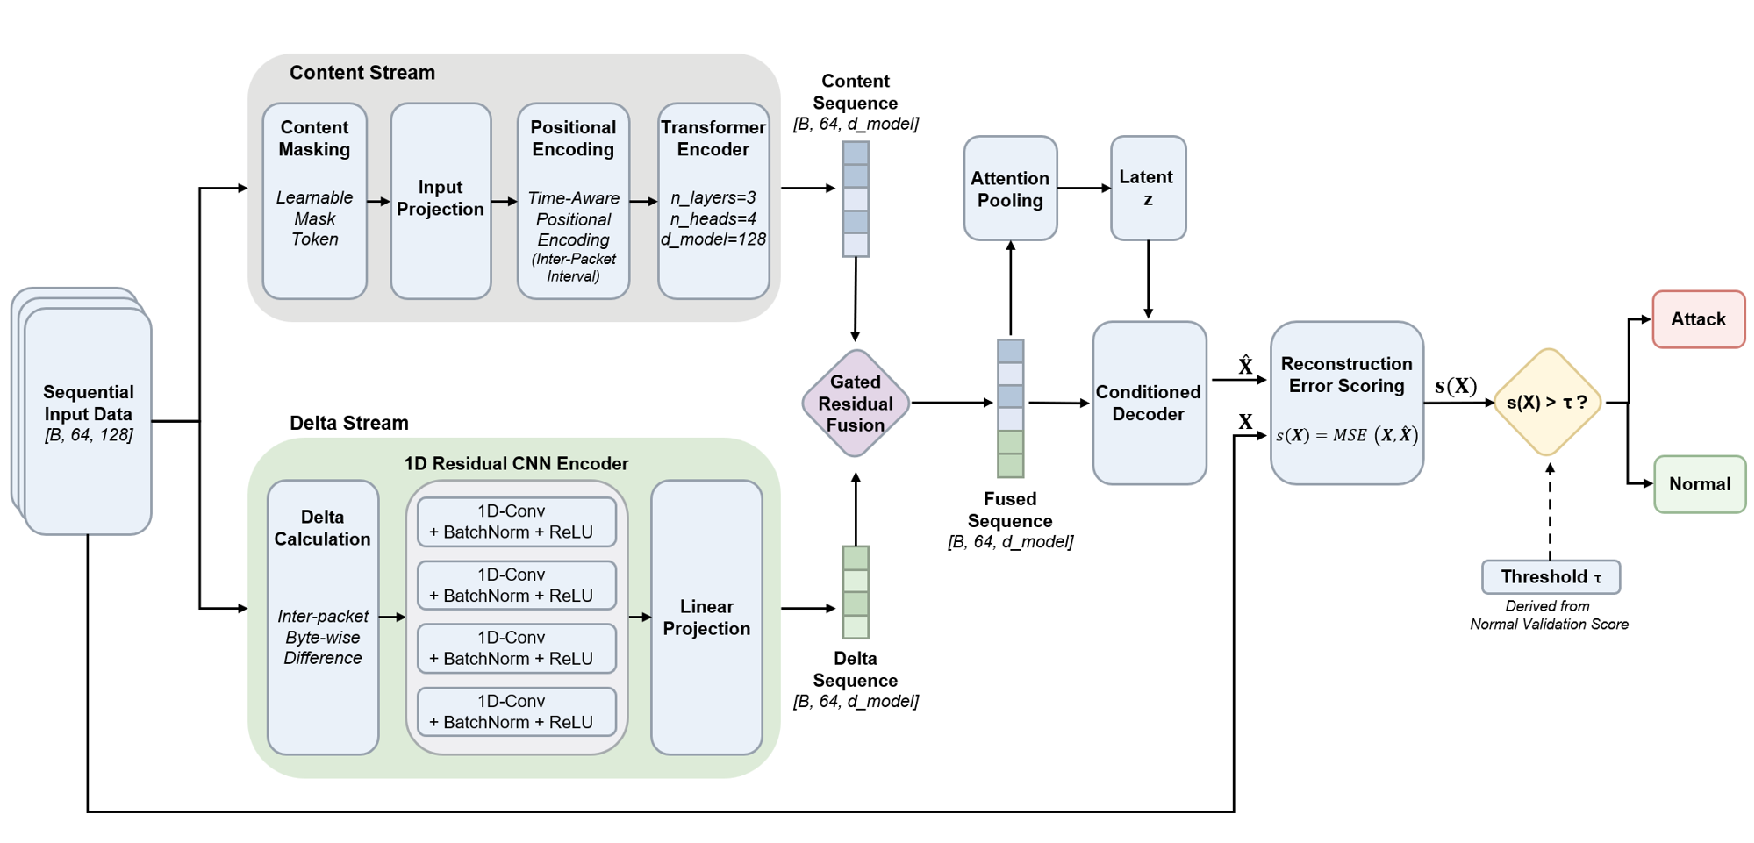
\includegraphics[width=\textwidth]{figs/architecture.pdf}
\caption{Overview of the proposed dual-stream masked autoencoder. The content stream (Transformer) is conditioned on both the masked packet content and a time-aware positional encoding derived from inter-packet capture timestamps; the delta stream (residual 1D-CNN) processes inter-packet byte differences. The two streams are combined through delta-conditioned gated residual fusion, after which attention pooling produces a global latent vector $\mathbf{z}$ that, together with the fused sequence representation $\mathbf{F}$, conditions the decoder's reconstruction. At inference, the mean reconstruction error $s(\mathbf{X})$ is compared against a validation-derived threshold $\tau$ to flag intrusions. Equation numbers refer to their first appearance in Section~\ref{sec:methodology}.}
\label{fig:architecture}
\end{figure*}

\subsection{Problem Formulation}
\begin{figure}[]
\centering
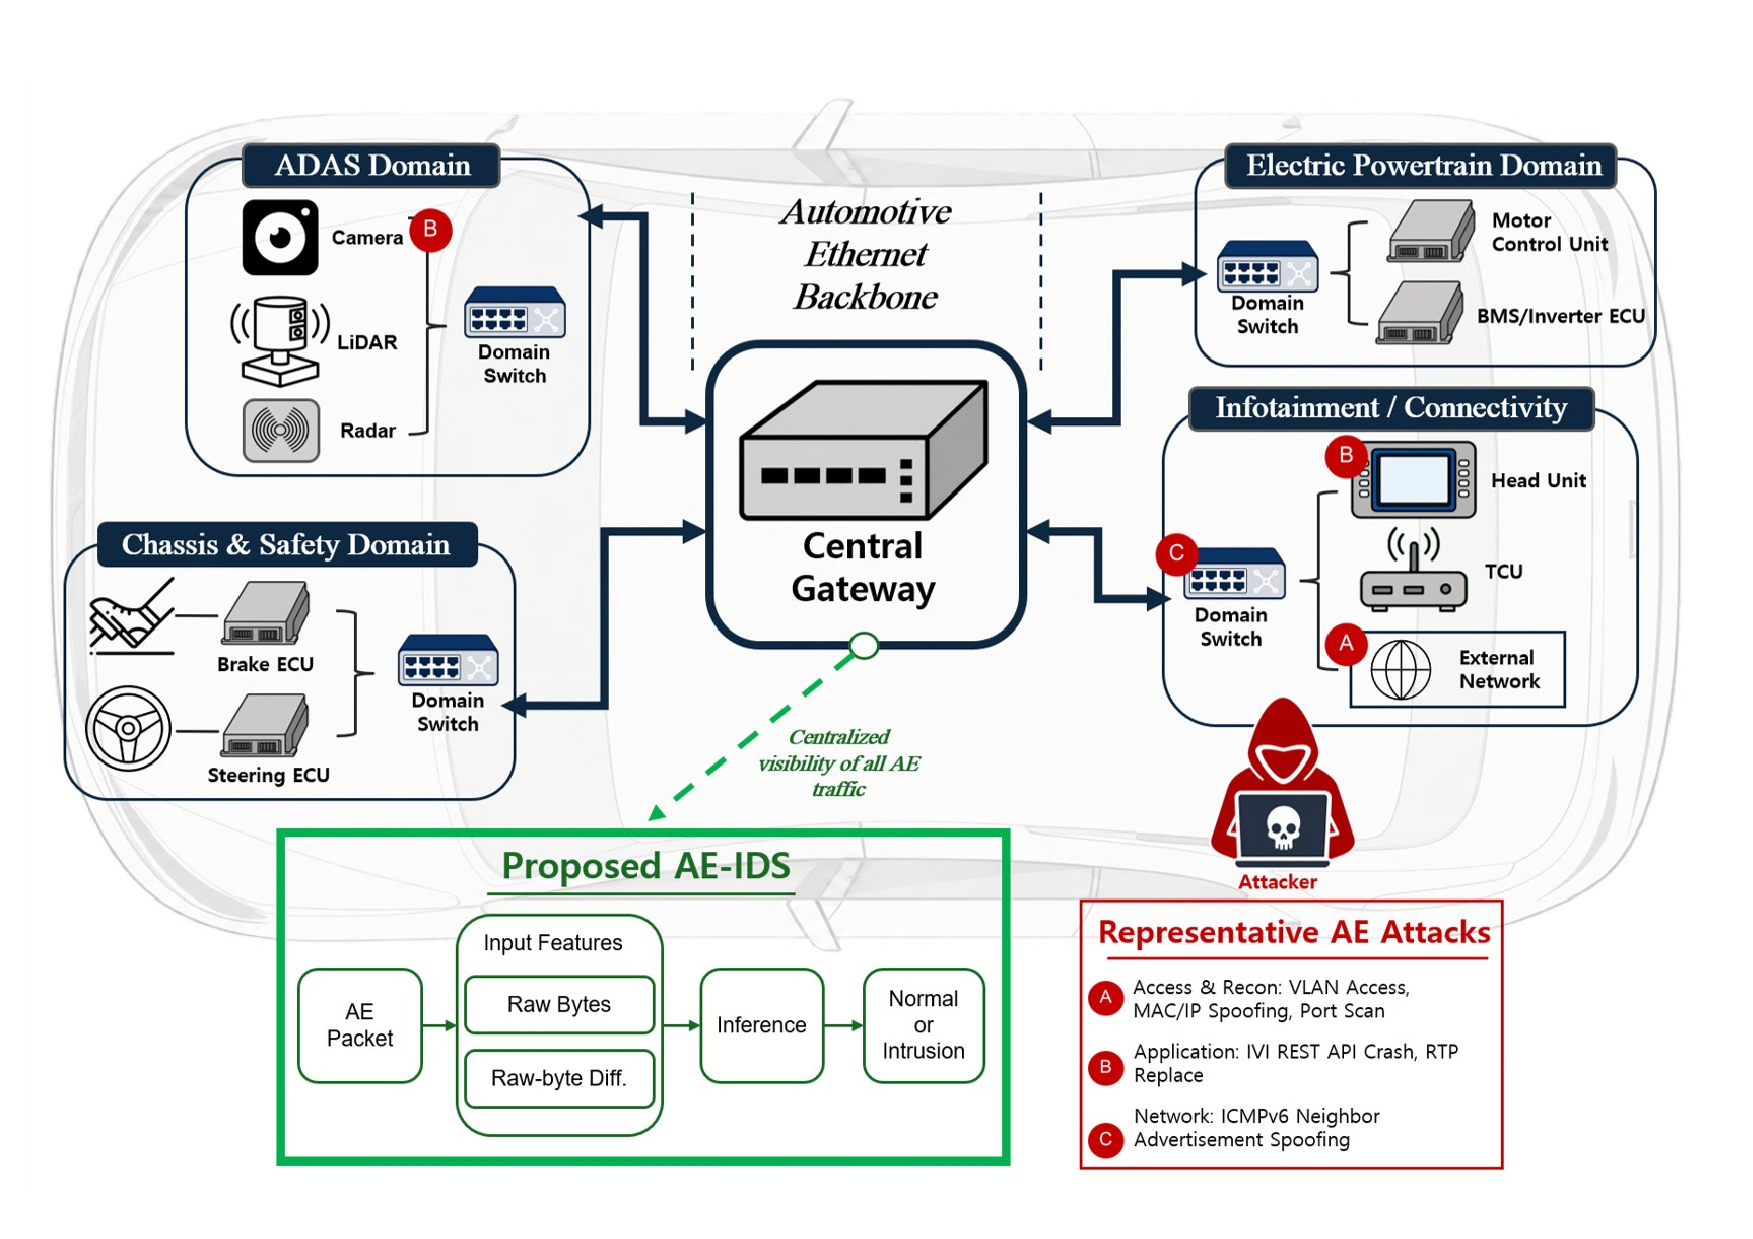
\includegraphics[width=\columnwidth]{figs/proposed_ids_architecture.pdf}
\caption{\textcolor{red}{Conceptual deployment of the proposed AE-IDS in a domain-based in-vehicle network. The ADAS, chassis and safety, electric powertrain, and infotainment/connectivity domains exchange inter-domain traffic through the Automotive Ethernet backbone and central gateway. The proposed detector passively analyzes gateway-visible AE packets using raw bytes and inter-packet raw-byte differences. The labeled markers summarize the representative CarDS attack scenarios considered in this work: (A) network access and reconnaissance, (B) application-layer exploitation, and (C) network-layer neighbor spoofing.}}
\label{fig:ae_deployment}
\end{figure}

\textcolor{red}{Figure~\ref{fig:ae_deployment} illustrates the intended deployment context of the proposed method. The four domains provide a conceptual functional partition of a modern electric vehicle rather than an exact reconstruction of a particular production topology. The ADAS domain contains high-bandwidth sensors, the chassis and safety domain contains safety-critical control ECUs, the electric powertrain domain contains the motor-control and battery/inverter ECUs, and the infotainment/connectivity domain contains the head unit, telematics control unit, and external-network interfaces. Their inter-domain AE traffic is forwarded through the central gateway, making the gateway a suitable centralized observation point for vehicle-wide intrusion detection.}

\textcolor{red}{The AE-IDS is assumed to receive a passive copy of the AE packets observable at the central gateway, for example through an internal monitoring interface, switch-port mirroring, or a passive tap. It therefore does not participate in packet forwarding and does not introduce additional control-path latency. The phrase \emph{centralized visibility} refers specifically to traffic that traverses, or is mirrored to, the gateway; traffic exchanged only within a local switched domain is observable only if the corresponding domain switch exports a copy to this monitoring point. This deployment assumption makes the monitoring coverage explicit while preserving the protocol-agnostic packet representation used by the detector.}

\textcolor{red}{The A--C markers in Figure~\ref{fig:ae_deployment} indicate where representative Automotive Ethernet attacks can enter or affect the network. Marker A denotes access and reconnaissance activity originating from the externally connected infotainment/connectivity domain, including unauthorized VLAN access, MAC/IP spoofing, and TCP port scanning. Marker B denotes the CarDS application-layer attacks: exploitation of an IVI REST API at the head unit and replacement of an unprotected RTP camera stream. The camera marker therefore represents the attacked video stream and does not imply that the same RTP-specific attack is directly applicable to LiDAR or radar traffic; attacks against those sensors would require protocol-specific injection or replay mechanisms. Marker C denotes forged ICMPv6 Neighbor Advertisement messages that manipulate the internal switch's neighbor/forwarding state and redirect traffic toward the attacker. Collectively, these attacks alter Ethernet headers, addressing and protocol fields, transport behavior, or application payloads. This motivates processing both the raw packet bytes and their consecutive byte-wise differences: the former preserves the complete packet content, while the latter emphasizes abrupt local changes introduced by spoofing, scanning, and frame replacement.}

We formulate Automotive Ethernet intrusion detection as an unsupervised anomaly detection problem. Let a raw packet be represented as a byte sequence $\mathbf{p}_i \in \{0, \ldots, 255\}^{L}$, where $L = 128$ denotes the maximum byte length, with zero-padding applied to packets shorter than $L$. Each byte value is normalized to $[0, 1]$ by dividing by 255. A traffic window is defined as a temporally ordered sequence of $N = 64$ consecutive packets, $\mathbf{X} = [\mathbf{p}_1, \mathbf{p}_2, \ldots, \mathbf{p}_N] \in \mathbb{R}^{N \times L}$, constructed using a sliding window of stride 1 over the full packet stream.

A window-level binary label $y \in \{0, 1\}$ is assigned during evaluation only: $y = 1$ if at least one packet within the window is malicious, and $y = 0$ otherwise. The model is trained exclusively on windows drawn from normal traffic ($y = 0$) and receives no label information during training. The objective is to learn a function $f: \mathbb{R}^{N \times L} \rightarrow \mathbb{R}_{\geq 0}$ that assigns a scalar anomaly score to each window such that anomalous windows receive systematically higher scores than normal windows. At inference time, a window is classified as an intrusion if its anomaly score exceeds a threshold $\tau$ derived from the normal traffic distribution.

\noindent\textit{Notational convention.} Throughout this section, all vector and matrix quantities follow the row-vector convention, in which a linear projection is written as $\mathbf{Y} = \mathbf{X}\mathbf{W} + \mathbf{b}$ with $\mathbf{W} \in \mathbb{R}^{d_{\text{in}} \times d_{\text{out}}}$. Sequence-level quantities (e.g., $\mathbf{X}, \mathbf{C}, \mathbf{D}, \mathbf{F}$) are treated as $N \times d$ matrices whose rows correspond to individual packets, while window-level quantities that collapse the sequence into a single vector (e.g., $\bar{\mathbf{z}}, \mathbf{z}$) are treated as $1 \times d$ row vectors under the same convention.



\subsection{Overview of the Proposed Method}
The proposed method consists of three components: (1) a dual-stream encoder that produces a latent representation of the input window, (2) a masked reconstruction objective used for self-supervised training, and (3) a threshold-based anomaly scoring mechanism used at inference time. An overview of the full architecture is shown in Figure~\ref{fig:architecture}.

The dual-stream encoder processes the input window $\mathbf{X}$ through two parallel streams. The \textbf{content stream} applies a Transformer encoder to the raw byte content of each packet, modeling global inter-packet dependencies across the full window; rather than the conventional fixed sinusoidal positional encoding, the content stream is conditioned on the actual inter-packet timing recorded at capture time, allowing it to reason jointly about packet content and packet timing. The \textbf{delta stream} applies a residual 1D-CNN encoder to the inter-packet byte difference sequence, modeling per-byte temporal dynamics across consecutive packets. The content stream serves as the primary carrier of discriminative information, while the delta stream acts as a self-gated auxiliary signal that supplements it with local temporal cues. The outputs of both streams are fused through a delta-conditioned gated residual mechanism and aggregated via attention pooling to produce a compact latent vector $\mathbf{z}$. A conditioned sequence decoder then reconstructs the original packet content from the fused sequence representation and $\mathbf{z}$. Table~\ref{tab:notation} summarizes the notation used throughout this section.

\begin{table}[!t]
\centering
\caption{Summary of notation.}
\label{tab:notation}
\footnotesize
\begin{tabular}{cp{0.7\columnwidth}}
\toprule
\textbf{Symbol} & \textbf{Description} \\
\midrule
$N, L$                          & window size (64), byte length (128) \\
$\mathbf{p}_i$                  & raw content of packet $i$ \\
$\mathbf{\Delta X}_i$           & inter-packet byte difference at $i$ \\
$\iota_i$                       & inter-packet interval (IPI) at $i$ \\
$\mathbf{m}, m_i$                & packet-level mask vector / indicator \\
$\mathbf{e}_{\text{mask}}$      & learnable mask token \\
$\mathbf{P}, \mathbf{T}$        & sinusoidal, time-aware positional encoding \\
$\mathbf{C}, \mathbf{D}$        & content-, delta-stream outputs \\
$\mathbf{F}$                    & fused sequence representation \\
$\bar{\mathbf{z}}, \mathbf{z}$  & pooled, refined latent vector \\
$\hat{\mathbf{p}}_i$            & reconstructed content of packet $i$ \\
$\tau$                          & anomaly detection threshold \\
\bottomrule
\end{tabular}
\end{table}

\subsection{Input Representation}

\noindent\textbf{Raw Content Input.}
The content stream receives the normalized window $\mathbf{X} \in \mathbb{R}^{N \times L}$ directly as input, where each row $\mathbf{p}_i \in \mathbb{R}^{L}$ represents the normalized byte content of the $i$-th packet.

\noindent\textbf{Delta Input.}
The delta stream receives the inter-packet byte difference sequence $\mathbf{\Delta X} \in \mathbb{R}^{N \times L}$, computed as
\begin{equation}
    \mathbf{\Delta X}_i =
    \begin{cases}
        \mathbf{0} & \text{if } i = 1 \\
        \mathbf{p}_i - \mathbf{p}_{i-1} & \text{if } i > 1.
    \end{cases}
    \label{eq:delta}
\end{equation}
The delta sequence captures how each byte position evolves across consecutive packets. Under normal traffic, protocol fields such as sequence numbers exhibit predictable incremental patterns; anomalous traffic introduces irregular byte-level fluctuations at specific positions that are more salient in the delta domain than in the raw content domain.

\noindent\textbf{Temporal Input.}
In addition to byte-level content and delta, we incorporate inter-packet timing as a third input modality. Let $t_i$ denote the capture timestamp of packet $i$. The inter-packet interval (IPI) sequence $\boldsymbol{\iota} \in \mathbb{R}^{N \times 1}$ is computed as
\begin{equation}
    \iota_i =
    \begin{cases}
        0 & \text{if } i = 1 \\
        \log\!\left(1 + |t_i - t_{i-1}|\right) & \text{if } i > 1,
    \end{cases}
    \label{eq:ipi}
\end{equation}

mirroring the zero-initialization convention used for the delta sequence [Eq.~\eqref{eq:delta}]. The logarithmic compression $\log(1+|\cdot|)$ accounts for the wide dynamic range of Automotive Ethernet inter-arrival times, which span several orders of magnitude (microseconds to seconds) depending on traffic type and driving scenario; without this compression, occasional large inter-arrival gaps would dominate the learned representation. The IPI sequence is derived solely from packet capture timestamps and is independent of any upper-layer protocol parsing, preserving the protocol-agnostic nature of the proposed method.

\noindent\textbf{Masking.}
Prior to encoding, a packet-level binary mask $\mathbf{m} \in \{0, 1\}^{N}$ is sampled to determine which packets within the window are masked: each position $i \in \{1, \ldots, N\}$ is independently drawn as $m_i \sim \text{Bernoulli}(p_{\text{mask}})$ with $p_{\text{mask}} = 0.20$, so that approximately 20\% of the $N$ packets in each window are selected for masking. For each position where $m_i = 1$, the entire $L$-dimensional content vector $\mathbf{p}_i$ is replaced --- not with random values, but with a single shared, learned mask token $\mathbf{e}_{\text{mask}} \in \mathbb{R}^{L}$, initialized from $\mathcal{N}(0, 0.02^2)$ and updated during training via backpropagation:
\begin{equation}
    \tilde{\mathbf{p}}_i =
    \begin{cases}
        \mathbf{e}_{\text{mask}} & \text{if } m_i = 1 \\
        \mathbf{p}_i             & \text{if } m_i = 0.
    \end{cases}
    \label{eq:mask}
\end{equation}

This design follows the masked autoencoding paradigm of BERT~\cite{devlin2019bert} and MAE~\cite{he2022masked}, where the \emph{location} of masking is randomized while the \emph{substituted value} is a single learnable embedding shared across all masked positions, rather than random noise. The delta input is computed from the original unmasked content [Eq.~\eqref{eq:delta}] and is not subject to masking, preserving the integrity of the variation signal. Similarly, the IPI sequence $\boldsymbol{\iota}$ [Eq.~\eqref{eq:ipi}] is left unmasked at every position, including $i$ with $m_i = 1$: only the byte-level content vector $\mathbf{p}_i$ is replaced by $\mathbf{e}_{\text{mask}}$, while the timing signal used to compute $\mathbf{P}_{\text{enc}}$ remains the true inter-packet interval. This mirrors standard practice in masked autoencoding architectures, where positional encodings are treated as always-visible structural context rather than maskable content; masking the timing signal itself would additionally confound the reconstruction objective, since the decoder would then have to infer both the missing content and the missing timing of a packet from a single shared mask token.

\subsection{Dual-Stream Encoder}
\subsubsection{Content Stream: Transformer Encoder}
The content stream models global inter-packet dependencies using a standard Transformer encoder~\cite{vaswani2017attention}. Let $\tilde{\mathbf{X}} = [\tilde{\mathbf{p}}_1, \ldots, \tilde{\mathbf{p}}_N]$ denote the masked window from Eq.~\eqref{eq:mask}. The masked content input is first projected to the model dimension $d_{\text{model}} = 128$ via a linear layer, after which a positional encoding matrix $\mathbf{P}_{\text{enc}} \in \mathbb{R}^{N \times d_{\text{model}}}$ is added to inject positional information:
\begin{equation}
    \mathbf{H}^{(0)}_c = \text{Dropout}\!\left( \tilde{\mathbf{X}}\mathbf{W}_c + \mathbf{b}_c + \mathbf{P}_{\text{enc}} \right) \in \mathbb{R}^{N \times d_{\text{model}}},
    \label{eq:posenc}
\end{equation}

where $\mathbf{W}_c \in \mathbb{R}^{L \times d_{\text{model}}}$ is the projection weight and $\text{Dropout}(\cdot)$ is applied at rate $p_{\text{drop}} = 0.1$. The same rate $p_{\text{drop}} = 0.1$ is used uniformly across the network: in Eq.~\eqref{eq:posenc} above, inside each Transformer encoder layer of Eq.~\eqref{eq:transformer}, and in the latent refinement step of Eq.~\eqref{eq:latent}. We consider two schemes for instantiating $\mathbf{P}_{\text{enc}}$, compared directly in the ablation study of Section~\ref{sec:ablation}.

\noindent\textit{Sinusoidal positional encoding (baseline).} Following the conventional Transformer scheme~\cite{vaswani2017attention}, $\mathbf{P}_{\text{enc}} = \mathbf{P}$ is a fixed matrix computed from each packet's discrete rank $i \in \{1, \ldots, N\}$ within the window using the standard sine/cosine basis. This scheme encodes only the \emph{ordinal position} of a packet (0th, 1st, \ldots, 63rd) and is invariant to the actual elapsed time between packets.

\noindent\textit{Time-aware positional encoding (proposed).} Automotive Ethernet attacks such as high-rate port scanning, packet replay, and flooding typically manifest as anomalous \emph{inter-arrival timing} rather than anomalous sequence rank, a signal that the sinusoidal scheme cannot represent. We therefore propose conditioning the positional signal directly on the IPI sequence $\boldsymbol{\iota}$ [Eq.~\eqref{eq:ipi}] via a learnable projection:
\begin{equation}
    \mathbf{P}_{\text{enc}} = \mathbf{T} =
    \text{GELU}\!\left(\boldsymbol{\iota}\mathbf{W}_{t_1} + \mathbf{b}_{t_1}\right)\mathbf{W}_{t_2} + \mathbf{b}_{t_2},
    \label{eq:timepe}
\end{equation}

with $\mathbf{T} \in \mathbb{R}^{N \times d_{\text{model}}}$, $\mathbf{W}_{t_1} \in \mathbb{R}^{1 \times d_{\text{model}}}$ and $\mathbf{W}_{t_2} \in \mathbb{R}^{d_{\text{model}} \times d_{\text{model}}}$. Unlike the fixed sinusoidal matrix $\mathbf{P}$, the time-aware encoding $\mathbf{T}$ is differentiable and learns to map raw timing irregularities directly into the representation space, replacing ``\emph{which position is this packet}'' with ``\emph{how much time elapsed before this packet arrived}'' as the positional signal injected into the content stream. Unless otherwise noted, the time-aware scheme is adopted as the default configuration for the results reported in this paper; the sinusoidal scheme is retained as an ablation baseline to isolate its contribution.

The projected sequence $\mathbf{H}^{(0)}_c$ is passed through $n_{\text{layers}} = 3$ Transformer encoder layers with pre-layer normalization, each consisting of multi-head self-attention with $n_{\text{head}} = 4$ heads and a position-wise feed-forward network with hidden dimension $d_{\text{ff}} = 256$:
\begin{equation}
    \mathbf{C} = \text{TransformerEncoder}(\mathbf{H}^{(0)}_c) \in \mathbb{R}^{N \times d_{\text{model}}}.
    \label{eq:transformer}
\end{equation}

The Transformer encoder is suited to the content stream because inter-packet dependencies in Automotive Ethernet traffic are inherently global: the anomalous nature of a given packet may be most apparent in relation to temporally distant packets, such as when a scanning sequence targets non-consecutive port ranges across the window. This global receptive field also motivates injecting timing information specifically into the content stream rather than the delta stream: because self-attention computes interactions among all $N$ packets jointly, an anomalously short or long inter-packet interval can be weighed by attention relative to the timing of every other packet in the window. In contrast, the delta stream's convolutional kernels (size 3--5) only relate a packet to its immediate neighbors, limiting their ability to contextualize timing irregularities against the full window.

\subsubsection{Delta Stream: Residual CNN Encoder}
The delta stream captures local temporal change patterns at each byte position using a residual one-dimensional convolutional neural network. Since each byte position across $N$ consecutive packets constitutes an independent temporal signal, the delta sequence $\mathbf{\Delta X} \in \mathbb{R}^{N \times L}$ from Eq.~\eqref{eq:delta} is transposed to $\mathbb{R}^{L \times N}$, treating each byte position as a channel and the packet index as the sequence axis. The transposed input is processed by a stack of residual convolutional blocks with filter progression $[128, 128, 128, C_{\text{last}}]$, $C_{\text{last}} = 64$:
\begin{equation}
    \mathbf{D}' = \text{ResidualCNN}\!\left(\mathbf{\Delta X}^{\top}\right) \in \mathbb{R}^{C_{\text{last}} \times N}.
    \label{eq:cnn}
\end{equation}

Each residual block applies two successive 1D convolutions with kernel size 3 (kernel size 5 in the final block), batch normalization, and ReLU activation, with a $1\times1$ convolutional skip connection applied whenever the input and output channel dimensions differ. Formally, letting $\mathbf{U}^{(l-1)}$ denote the input to the $l$-th block ($\mathbf{U}^{(0)} = \mathbf{\Delta X}^{\top}$), each block computes
{\footnotesize
\begin{multline}
    \mathbf{U}^{(l)} = \text{ReLU}\!\Big(\text{BN}\big(\text{Conv}_2^{(l)}(\text{ReLU}(\text{BN}(\text{Conv}_1^{(l)}(\mathbf{U}^{(l-1)}))))\big) \\
    {}+ \mathbf{S}^{(l)}\big(\mathbf{U}^{(l-1)}\big)\Big),
    \label{eq:resblock}
\end{multline}
}
where $\text{Conv}_1^{(l)}, \text{Conv}_2^{(l)}$ are the block's two 1D convolutions, $\text{BN}(\cdot)$ denotes batch normalization, and $\mathbf{S}^{(l)}(\cdot)$ is the skip path: the identity map if the input and output channel dimensions of block $l$ match, and a $1\times1$ convolution followed by batch normalization otherwise. Stacking $n_{\text{blocks}} = 4$ such blocks with channel progression $[128, 128, 128, C_{\text{last}}]$ ($C_{\text{last}} = 64$) yields $\mathbf{D}' = \mathbf{U}^{(n_{\text{blocks}})}$, consistent with the $\text{ResidualCNN}(\cdot)$ notation of Eq.~\eqref{eq:cnn} above. The output is then transposed back to sequence-first format and linearly projected to $d_{\text{model}}$:
\begin{equation}
    \mathbf{D} = {\mathbf{D}'}^{\top}\mathbf{W}_d + \mathbf{b}_d \in \mathbb{R}^{N \times d_{\text{model}}},
    \label{eq:deltaproj}
\end{equation}

where $\mathbf{W}_d \in \mathbb{R}^{C_{\text{last}} \times d_{\text{model}}}$ and $\mathbf{b}_d \in \mathbb{R}^{d_{\text{model}}}$.
This design allows the CNN to independently track how each byte position evolves over the packet sequence. By applying convolutional kernels along the packet axis with a local receptive field, the model efficiently detects position-specific anomalies --- such as irregular fluctuations in byte offsets corresponding to source addresses, port numbers, or RTP sequence fields --- that manifest as abrupt local deviations in the delta domain.

\begin{algorithm}[!t]
\caption{Self-Supervised Dual-Stream Masked Reconstruction Training}
\label{alg:training}
\begin{algorithmic}[1]
\REQUIRE Normal traffic windows $\{\mathbf{X}^{(k)}\}_{k=1}^{K_{\text{train}}}$, mask probability $p_{\text{mask}}$, masked-loss weight $\lambda$, max epochs $E$, patience $P$
\ENSURE Trained encoder-decoder parameters $\theta^\star$
\STATE Initialize model parameters $\theta$, including mask token $\mathbf{e}_{\text{mask}} \sim \mathcal{N}(0, 0.02^2)$
\STATE $b_{\text{best}} \gets \infty$; $c \gets 0$
\FOR{epoch $= 1$ \TO $E$}
    \FOR{each mini-batch $\{\mathbf{X}^{(k)}\}$ from training set}
        \STATE Compute delta sequence $\mathbf{\Delta X}^{(k)}$ via Eq.~\eqref{eq:delta} and IPI sequence $\boldsymbol{\iota}^{(k)}$ via Eq.~\eqref{eq:ipi}
        \STATE Sample packet-level mask $\mathbf{m}^{(k)} \sim \text{Bernoulli}(p_{\text{mask}})$ and apply Eq.~\eqref{eq:mask}
        \STATE Encode content stream $\mathbf{C}$ [Eqs.~\eqref{eq:posenc}--\eqref{eq:transformer}, with $\mathbf{P}_{\text{enc}} = \mathbf{T}$ from Eq.~\eqref{eq:timepe}] and delta stream $\mathbf{D}$ [Eq.~\eqref{eq:deltaproj}]
        \STATE Fuse streams into $\mathbf{F}$ via gated residual fusion [Eqs.~\eqref{eq:gate}--\eqref{eq:fusion}]
        \STATE Compute latent vector $\mathbf{z}$ via attention pooling and refinement [Eqs.~\eqref{eq:attnpool}--\eqref{eq:latent}]
        \STATE Decode reconstruction $\hat{\mathbf{X}}^{(k)}$ via Eq.~\eqref{eq:decoder}
        \STATE Compute loss $\mathcal{L}$ via Eq.~\eqref{eq:loss}; update $\theta$ with AdamW
    \ENDFOR
    \STATE Evaluate average validation loss $\mathcal{L}_{\text{val}}$ (masking applied with a fixed random seed)
    \IF{$\mathcal{L}_{\text{val}} < b_{\text{best}}$}
        \STATE $b_{\text{best}} \gets \mathcal{L}_{\text{val}}$; $\theta^\star \gets \theta$; $c \gets 0$
    \ELSE
        \STATE $c \gets c + 1$; \textbf{if} $c \geq P$ \textbf{then break}
    \ENDIF
\ENDFOR
\RETURN $\theta^\star$
\end{algorithmic}
\end{algorithm}

\subsubsection{Gated Residual Fusion}
\label{sec:fusion}
The content representation $\mathbf{C}$ [Eq.~\eqref{eq:transformer}] and delta representation $\mathbf{D}$ [Eq.~\eqref{eq:deltaproj}] are combined through a delta-conditioned gated residual mechanism. A gate is computed from the delta representation alone and used to modulate its contribution to the content representation:
\begin{equation}
    \mathbf{g} = \sigma\!\left(\mathbf{D}\mathbf{W}_g + \mathbf{b}_g\right) \in \mathbb{R}^{N \times d_{\text{model}}},
    \label{eq:gate}
\end{equation}
\begin{equation}
    \mathbf{F} = \mathbf{C} + \mathbf{g} \odot \mathbf{D} \in \mathbb{R}^{N \times d_{\text{model}}},
    \label{eq:fusion}
\end{equation}

where $\sigma(\cdot)$ denotes the sigmoid activation, $\mathbf{W}_g \in \mathbb{R}^{d_{\text{model}} \times d_{\text{model}}}$ is a learned weight matrix, and $\odot$ denotes element-wise multiplication. By conditioning the gate on the delta representation itself, the mechanism suppresses the delta stream's contribution at positions where inter-packet variation is uninformative, allowing the content stream to dominate when global sequential structure is the primary discriminative signal.

This formulation reflects a primary--auxiliary design rationale rather than a symmetric two-stream fusion: the content representation $\mathbf{C}$ constitutes the principal discriminative signal, capturing the global structure of packet content across the window, while the delta representation $\mathbf{D}$ serves as a supplementary correction that injects local temporal variation into $\mathbf{C}$ only where such variation is itself informative. Because $\mathbf{D}$ already enters the fusion additively as a correction term in Eq.~\eqref{eq:fusion}, its own magnitude provides a natural, parameter-efficient proxy for how much auxiliary information it should contribute, without requiring a heavier gate jointly conditioned on $[\mathbf{C} \,\|\, \mathbf{D}]$. We adopt this asymmetric, delta-conditioned gating in place of symmetric content--delta gating to keep the fusion mechanism lightweight while preserving the content stream's role as the primary carrier of discriminative information throughout the encoder.

The fused sequence representation $\mathbf{F}$ serves as the input to both attention pooling (Section~\ref{sec:pooling}) and the decoder (Section~\ref{sec:decoder}).

\subsection{Attention Pooling and Latent Representation}
\label{sec:pooling}
The fused sequence representation $\mathbf{F}$ is aggregated into a fixed-dimensional pooled vector $\bar{\mathbf{z}} \in \mathbb{R}^{d_{\text{model}}}$ via attention pooling:
\begin{equation}
    \alpha_i = \frac{\exp\!\left(s(\mathbf{F}_i)\right)}{\sum_{j=1}^{N} \exp\!\left(s(\mathbf{F}_j)\right)}, \qquad
    \bar{\mathbf{z}} = \sum_{i=1}^{N} \alpha_i \mathbf{F}_i,
    \label{eq:attnpool}
\end{equation}
where $s(\cdot): \mathbb{R}^{d_{\text{model}}} \rightarrow \mathbb{R}$ is a learned scoring function implemented as a two-layer MLP with a hidden dimension of $d_{\text{model}}/2 = 64$ and a Tanh nonlinearity. Attention pooling allows the model to assign non-uniform importance weights to individual packets when forming the global window representation, emphasizing packets that are most informative for characterizing normal traffic structure.

The pooled vector $\bar{\mathbf{z}}$ is further refined into the final latent vector $\mathbf{z} \in \mathbb{R}^{d_{\text{model}}}$ through a feed-forward refinement block consisting of a linear projection, layer normalization, ReLU activation, and dropout:
\begin{equation}
    \mathbf{z} = \text{Dropout}\!\left(\text{ReLU}\!\left(\text{LayerNorm}\!\left(\bar{\mathbf{z}}\mathbf{W}_z + \mathbf{b}_z\right)\right)\right),
    \label{eq:latent}
\end{equation}
where $\mathbf{W}_z \in \mathbb{R}^{d_{\text{model}} \times d_{\text{model}}}$.

\subsection{Conditioned Sequence Decoder}
\label{sec:decoder}
The decoder reconstructs the original (unmasked) packet content from the fused sequence representation $\mathbf{F}$ [Eq.~\eqref{eq:fusion}], conditioned on the global latent vector $\mathbf{z}$ [Eq.~\eqref{eq:latent}]. For each position $i$, the latent vector is broadcast and concatenated with the local sequence representation:
\begin{equation}
    \hat{\mathbf{p}}_i = \text{GELU}\!\left(\left[\mathbf{F}_i \,\|\, \mathbf{z}\right] \mathbf{W}_1 + \mathbf{b}_1\right) \mathbf{W}_2 + \mathbf{b}_2,
    \label{eq:decoder}
\end{equation}
where $[\,\cdot\,\|\,\cdot\,]$ denotes concatenation along the feature dimension, $\mathbf{W}_1 \in \mathbb{R}^{2d_{\text{model}} \times d_{\text{model}}}$ projects the concatenated input to $d_{\text{model}}$, and $\mathbf{W}_2 \in \mathbb{R}^{d_{\text{model}} \times L}$ maps to the output byte dimension.

Conditioning every position on the shared global latent $\mathbf{z}$ allows the decoder to reconstruct each packet using both its local fused context $\mathbf{F}_i$ and a summary of the entire window, which is particularly important for recovering masked positions that retain no local information of their own. The reconstructed window is denoted $\hat{\mathbf{X}} = [\hat{\mathbf{p}}_1, \ldots, \hat{\mathbf{p}}_N] \in \mathbb{R}^{N \times L}$.

\subsection{Training Objective}
\label{sec:loss}
The model is trained using a packet-level masked reconstruction loss with asymmetric weighting that emphasizes the reconstruction of masked positions:
\begin{equation}
    \mathcal{L} = \frac{\displaystyle\sum_{i=1}^{N} w_i \cdot \frac{1}{L} \left\| \hat{\mathbf{p}}_i - \mathbf{p}_i \right\|^2}{\displaystyle\sum_{i=1}^{N} w_i}, \qquad
    w_i =
    \begin{cases}
        \lambda & \text{if } m_i = 1 \\
        1       & \text{if } m_i = 0,
    \end{cases}
    \label{eq:loss}
\end{equation}
with $\lambda = 5.0$. The asymmetric weighting in Eq.~\eqref{eq:loss} encourages the model to devote greater representational capacity to recovering masked content, rather than trivially minimizing error at unmasked positions. Reconstruction of both masked and unmasked positions is retained in the loss to prevent degenerate solutions in which the encoder ignores unmasked context entirely.

The model is optimized using AdamW~\cite{loshchilov2019decoupled} with weight decay $10^{-4}$ and initial learning rate $\eta = 10^{-4}$, annealed via cosine scheduling to $\eta_{\min} = 10^{-6}$ over the full training schedule. Gradient norms are clipped at 1.0 to stabilize training, and early stopping is applied with a patience of 15 epochs, monitored on validation reconstruction loss. Algorithm~\ref{alg:training} summarizes the complete self-supervised training procedure.

\subsection{Anomaly Scoring and Threshold Determination}
\label{sec:scoring}

\noindent\textbf{Anomaly Score.}
At inference time, the trained model $f_{\theta^\star}$ performs a forward pass without masking ($\mathbf{m} = \mathbf{0}$). The anomaly score for a window $\mathbf{X}$ is defined as the mean per-packet reconstruction error:
\begin{equation}
    s(\mathbf{X}) = \frac{1}{N} \sum_{i=1}^{N} \frac{1}{L} \left\| \hat{\mathbf{p}}_i - \mathbf{p}_i \right\|^2.
    \label{eq:score}
\end{equation}

\noindent\textbf{Threshold Determination.}
The detection threshold $\tau$ is determined from the reconstruction error distribution of normal validation traffic, computed once after training using Eq.~\eqref{eq:score} over all $K$ validation windows without masking:
\begin{equation}
    \tau = \operatorname{Percentile}_{p}\!\left(\left\{s\!\left(\mathbf{X}^{(k)}\right)\right\}_{k=1}^{K}\right).
    \label{eq:threshold}
\end{equation}
A window is classified as an intrusion if $s(\mathbf{X}) > \tau$. We evaluate percentile values $p \in \{90, 95, 97, 99, 99.5, 99.9\}$ and select $p = 99$ based on the precision--recall tradeoff observed on the validation error distribution, which exhibits a sharp concentration of normal traffic errors near zero with a long right tail. The sensitivity of detection performance to the choice of $p$ is analyzed in Section~\ref{sec:threshold}.

We note that, while the model is trained in a fully unsupervised manner using only unlabeled normal traffic, identifying which percentile $p$ maximizes F1-score among the candidates above was performed using labeled attack data, consistent with common practice in unsupervised anomaly detection. In settings where labeled attacks are unavailable even for threshold calibration, $p$ may instead be selected using only the normal-traffic error distribution and a target false-positive rate (e.g., $p = 95$ for an intended 5\% FPR on validation traffic); Section~\ref{sec:threshold} reports detection performance under this fully label-free alternative, showing that it incurs only a modest reduction in F1-score relative to the labeled-calibration optimum.
\section{Experiments}
\label{sec:experiments}
\subsection{Dataset}
We evaluate the proposed method using the Automotive Ethernet traffic from the Controller Area Network and Automotive Ethernet Realistic Data Set (CarDS)~\cite{hellemans2025cards}. CarDS was collected from a commercial electric vehicle manufactured in 2020 and contains time-synchronized traffic from six AE links connecting the gateway electronic control unit (ECU), denoted GWE, to various vehicle components, including the rear-view camera, communication ECUs, and in-vehicle infotainment (IVI) system. In this work, we use the AE traces provided in PCAPNG format, in which attack packets are annotated through packet comments.

The AE traffic was captured using a breakout box installed between the GWE and the AE-connected ECUs. Since CarDS simultaneously records traffic from multiple AE links, a packet propagated through the GWE may be observed more than once. We therefore remove duplicate packet observations caused by GWE propagation from both benign and attack traces before preprocessing and window generation.

For training and validation, we use all 39 benign AE traces provided by CarDS. These traces cover four vehicle operating conditions: standstill, slow driving below 10\,km/h, fast driving above 10\,km/h, and reverse driving. The traces were collected at two restricted sites: a university private parking lot (PPL) and a driving school test area (DSTA). The DSTA emulates public-road conditions through traffic lights, traffic signs, intersections, and roundabouts. Thus, the benign traces capture variations in normal AE traffic across different driving conditions, vehicle states, and recording environments.

We use 31 benign traces for training and the remaining eight for validation. After duplicate removal, preprocessing, and window generation, the training and validation sets contain 5,433,175 and 3,066,673 normal windows, respectively. Sliding windows are constructed independently for each trace, ensuring that no window spans packets from different traces.

CarDS provides 31 Ethernet attack traces, of which 27 are used for performance evaluation. The selected traces comprise five RTP stream replacement traces and 22 Nmap scanning and spoofing traces. The RTP stream replacement attack substitutes frames in the unprotected rear-view camera stream with attacker-controlled video frames. The corresponding traces were recorded under reverse-driving, slow-driving, and standstill conditions.

The Nmap traces target the IVI and emergency communication ECUs and include SYN (\texttt{-sS}), ACK (\texttt{-sA}), and FIN (\texttt{-sF}) scans. The traces cover different port ranges and attacker configurations, including MAC spoofing, IP spoofing, combined MAC and IP spoofing, invalid IP addresses, and VLAN IDs 3 and 4.

Four traces in which attack packets account for no more than $0.01\%$ of all packets are excluded from the performance evaluation: \path{IVI-Nmap_sA_p49000_50000}, \path{IVI-Nmap_sF_p49000_50000}, \path{IVI-Nmap_sS_p1_1024}, and \path{IVI-RestAPI_Crash_vlan3}. These traces contain too few attack samples relative to benign traffic to support a reliable performance evaluation. Table~\ref{tab:dataset} summarizes the experimental dataset constructed from the CarDS AE traces after duplicate removal, preprocessing, and trace-wise sliding-window generation.

\begin{table}[!htbp]
\centering
\caption{Statistics of the experimental dataset constructed from CarDS
AE traces after deduplication and preprocessing.}
\label{tab:dataset}
\footnotesize
\adjustbox{max width=\columnwidth}{%
\begin{tabular}{lrrr}
\toprule
\textbf{Split} & \textbf{Files} & \textbf{Windows} & \textbf{Anomalous} \\
\midrule
Training (normal)           & 31 & 5,433,175 & 0 \\
Validation (normal)         &  8 & 3,066,673 & 0 \\
\midrule
RTP Stream Replacement      &  5 & 1,291,777 &   301,173 \\
Nmap Scanning \& Spoofing   & 22 & 3,811,885 & 1,998,714 \\
\textbf{Total Attack Files} & \textbf{27} & \textbf{5,103,662} & \textbf{2,299,887} \\
\bottomrule
\end{tabular}}
\end{table}

\subsection{Experimental Setup}
\label{sec:experimental_setup}
\noindent\textbf{Implementation Details.}
The proposed model is implemented in PyTorch~\cite{pytorch} and trained for up to 50 epochs with early stopping (patience = 15 epochs) based on validation reconstruction loss. Training is performed on NVIDIA GeForce RTX 3070 and RTX 3080 GPUs. The model is trained exclusively on normal traffic; no labeled attack samples are used at any stage of training. Input representations and the training objective follow the definitions in Section~\ref{sec:methodology}: inputs are preprocessed as specified in Eqs.~\eqref{eq:delta}--\eqref{eq:mask}, and the model is optimized using the asymmetric masked reconstruction loss (Eq.~\ref{eq:loss}) with $\lambda = 5.0$ and $p_{\text{mask}} = 0.20$. The core architecture and training hyperparameters are listed in Table~\ref{tab:hyperparams}.

\noindent\textbf{Evaluation Protocol.}
Each test file is evaluated independently via sliding-window inference with stride 1, and window-level labels follow the any-positive convention: a window is labeled anomalous if at least one of its constituent packets is malicious. We report precision, recall, and F1-score for each attack file. Within each attack category, per-file results are summarized as a macro-averaged subtotal; an overall micro-averaged score is additionally computed by pooling predictions across all 27 attack files. The window-level F1-score serves as the primary metric, with precision and recall reported separately to characterize the precision--recall tradeoff. AUROC and AUPRC are additionally reported as threshold-independent metrics. Anomaly scoring and threshold determination follow the formulations in Section~\ref{sec:scoring} (Eqs.~\ref{eq:score}--\ref{eq:threshold}): a window is flagged as anomalous if its anomaly score $s(\mathbf{X})$ exceeds $\tau$. For a given percentile $p$, $\tau$ is computed solely from the benign validation set; the choice of $p$ itself is made against labeled attacks. In this evaluation $\tau$ is set to the 99th percentile of the validation anomaly score distribution, denoted $P_{99}$; Section~\ref{sec:threshold} motivates that choice and quantifies the cost of selecting $p$ without labels.

\begin{table}[!htbp]
\centering
\caption{Architecture and training hyperparameters used for the proposed method.}
\label{tab:hyperparams}
\footnotesize
\adjustbox{max width=\columnwidth}{%
\begin{tabular}{ll}
\toprule
\textbf{Hyperparameter} & \textbf{Value} \\
\midrule
Window size ($N$)                       & 64 packets \\
Byte length ($L$)                       & 128 bytes \\
Model dimension ($d_{\text{model}}$)    & 128 \\
Transformer layers                      & 3 \\
Attention heads                         & 4 \\
FFN hidden dimension                    & 256 \\
CNN filter progression                  & [128, 128, 128, 64] \\
Positional encoding                     & Time-aware (IPI-based) \\
Dropout rate ($p_{\text{drop}}$)        & 0.1 \\
Mask probability ($p_{\text{mask}}$)    & 0.20 \\
Masked loss weight ($\lambda$)          & 5.0 \\
Optimizer                               & AdamW \\
Learning rate ($\eta$)                  & $1 \times 10^{-4}$ \\
Minimum learning rate                   & $1 \times 10^{-6}$ \\
LR schedule                             & Cosine annealing \\
Weight decay                            & $1 \times 10^{-4}$ \\
Gradient clipping                       & 1.0 \\
Batch size                              & 64 \\
Max epochs ($E$)                        & 50 \\
Early stopping patience                 & 15 epochs \\
\bottomrule
\end{tabular}}
\end{table}

\subsection{Main Results}
\label{sec:main_results}
Table~\ref{tab:main_results} reports the detection performance of the proposed dual-stream masked autoencoder with time-aware positional encoding across all 27 attack files at the $P_{99}$ threshold. The method achieves an overall micro-averaged F1-score of 0.9808 (Precision: 0.9852, Recall: 0.9764; Table~\ref{tab:main_results}), with AUROC of 0.9974 and AUPRC of 0.9972 (Table~\ref{tab:rocprc}). The per-category \emph{Subtotal} rows report the macro-average across files within each category, while the \textbf{Overall} row is micro-averaged across all 27 files; the two aggregation schemes are not directly comparable (see Table~\ref{tab:main_results} caption).

\begin{table*}[!tbp]
\centering
\caption{Detection results of the proposed method (Transformer-CNN with time-aware positional encoding) across 27 attack files (threshold: $P_{99}$), grouped by \textbf{Category} (RTP vs.\ Nmap) and \textbf{Subcategory} (RTP Replace, or, within Nmap, the type of identity spoofing combined with the port scan: MAC, IP, MAC+IP, or none); port range is an experimental parameter and not used for grouping. RD/SD/SS: Reverse/Slow/Standstill driving. \emph{Subtotal} rows report macro-averaged (per-file mean) values within each category; \textbf{Overall} reports micro-averaged (pooled-window) values across all 27 files; the two are not directly comparable.}
\label{tab:main_results}
\footnotesize
\adjustbox{max width=\textwidth}{%
\begin{tabular}{lllccc}
\toprule
\textbf{Category} & \textbf{Subcategory} & \textbf{Attack File} & \textbf{Prec.} & \textbf{Recall} & \textbf{F1} \\
\midrule
\multirow[c]{6}{*}{RTP} & \multirow[c]{5}{*}{RTP Replace}
 & RD-University-RearCamera-ReplaceRTP\_1                    & 0.9270 & 0.9165 & 0.9217 \\
 & & RD-University-RearCamera-ReplaceRTP\_2                    & 0.8459 & 0.8080 & 0.8265 \\
 & & RD-University-RearCamera-ReplaceRTP\_3                    & 0.9317 & 0.8143 & 0.8690 \\
 & & SD-University-RearCamera-ReplaceRTP                       & 0.8531 & 0.8356 & 0.8443 \\
 & & SS-University-RearCamera-ReplaceRTP                       & 0.9349 & 0.8550 & 0.8932 \\
\addlinespace[2pt]
 & & \textit{Subtotal (macro)}                      & \textit{0.8985} & \textit{0.8459} & \textit{0.8709} \\
\midrule
\multirow[c]{26}{*}{Nmap} & \multirow[c]{8}{*}{MAC Spoofing}
 & SS-University-IVI-sA\_MACSpoofing\_vlan3\_1                  & 0.9981 & 0.9983 & 0.9982 \\
 & & SS-University-IVI-sA\_MACSpoofing\_vlan3\_2                  & 0.9996 & 0.9982 & 0.9989 \\
 & & SS-University-IVI-sA\_MACSpoofing\_vlan3\_3                  & 0.9997 & 0.9970 & 0.9984 \\
 & & SS-University-IVI-sS\_MACSpoofing\_vlan3\_1                  & 0.9974 & 0.9989 & 0.9982 \\
 & & SS-University-IVI-sS\_MACSpoofing\_vlan3\_2                  & 0.9994 & 0.9991 & 0.9993 \\
 & & SS-University-IVI-sS\_p49000\_50000\_MACSpoofing\_vlan3\_1   & 0.9623 & 0.9842 & 0.9731 \\
 & & SS-University-IVI-sS\_p49000\_50000\_MACSpoofing\_vlan3\_2   & 0.8864 & 0.9691 & 0.9259 \\
 & & SS-University-IVI-sS\_p49000\_50000\_MACSpoofing\_vlan3\_3   & 0.9419 & 0.9770 & 0.9591 \\
\addlinespace[2pt]
 & & \textit{Subtotal (macro)}                      & \textit{0.9731} & \textit{0.9902} & \textit{0.9814} \\
\cmidrule(l){2-6}
 & \multirow[c]{9}{*}{IP Spoofing}
 & SS-University-IVI-sA\_p49000\_50000\_IPSpoofing\_vlan3          & 0.9818 & 0.9921 & 0.9869 \\
 & & SS-University-Emergency-sS\_IPSpoofing\_vlan4\_1                & 0.9932 & 0.9197 & 0.9550 \\
 & & SS-University-Emergency-sS\_IPSpoofing\_vlan4\_2                & 0.9824 & 0.9519 & 0.9669 \\
 & & SS-University-Emergency-sS\_IPSpoofing\_vlan4\_3                & 0.9899 & 0.9504 & 0.9698 \\
 & & SS-University-Emergency-sS\_IPSpoofing\_vlan4\_4                & 0.9949 & 0.9642 & 0.9793 \\
 & & SS-University-Emergency-sS\_p49000\_50000\_IPSpoofing\_vlan4    & 0.9852 & 0.9138 & 0.9481 \\
 & & SS-University-IVI-sS\_p49000\_50000\_IPSpoofing\_vlan3\_1       & 0.9404 & 0.9816 & 0.9606 \\
 & & SS-University-IVI-sS\_p49000\_50000\_IPSpoofing\_vlan3\_2       & 0.9826 & 0.9920 & 0.9873 \\
 & & SS-University-IVI-sF\_p49000\_50000\_IPSpoofing\_vlan3          & 0.9905 & 0.9872 & 0.9889 \\
\addlinespace[2pt]
 & & \textit{Subtotal (macro)}                      & \textit{0.9823} & \textit{0.9614} & \textit{0.9714} \\
\cmidrule(l){2-6}
 & \multirow[c]{3}{*}{MAC+IP Spoofing}
 & SS-University-Emergency-sS\_p49000\_50000\_MACSpoofing\_IPSpoofing\_vlan4  & 0.9502 & 0.9464 & 0.9483 \\
 & & SS-University-IVI-sS\_MACSpoofing\_IPSpoofing\_InvalidIP\_vlan3            & 0.9998 & 0.9982 & 0.9990 \\
 & & SS-University-IVI-sS\_MACSpoofing\_IPSpoofing\_vlan3                       & 0.9924 & 0.9993 & 0.9958 \\
\addlinespace[2pt]
 & & \textit{Subtotal (macro)}                      & \textit{0.9808} & \textit{0.9813} & \textit{0.9810} \\
\cmidrule(l){2-6}
 & \multirow[c]{2}{*}{No Spoofing}
 & SS-University-Emergency-sS\_p8000\_10000\_vlan4          & 0.9928 & 0.9462 & 0.9689 \\
 & & SS-University-IVI-sS\_p49000\_50000\_vlan3               & 0.9369 & 0.9924 & 0.9639 \\
\addlinespace[2pt]
 & & \textit{Subtotal (macro)}                      & \textit{0.9649} & \textit{0.9693} & \textit{0.9664} \\
\midrule
\multicolumn{3}{l}{\textbf{Overall (micro)}} & \textbf{0.9852} & \textbf{0.9764} & \textbf{0.9808} \\
\bottomrule
\end{tabular}}
\end{table*}

\noindent\textbf{Nmap-based attacks.} The proposed method achieves near-perfect detection on Nmap-based scanning and spoofing attacks, with subcategory-level F1-scores ranging from 0.9664 to 0.9814 (Table~\ref{tab:main_results}). The MAC Spoofing subcategory yields the highest subcategory-level F1 (macro F1 = 0.9814), closely followed by MAC+IP Spoofing (macro F1 = 0.9810); the single best-performing file overall is a SYN-scan MAC spoofing capture (F1 = 0.9993). Detection remains robust even without any spoofing signal: the No Spoofing subcategory, comprising unmodified port scans, still achieves a macro-averaged F1 of 0.9664, the lowest among Nmap-based subcategories but still substantially above the RTP subcategory discussed below.

\noindent\textbf{RTP stream replacement attacks.} Detection of RTP stream replacement attacks remains the most challenging subcategory, with a macro-averaged F1 of 0.8709 (Table~\ref{tab:main_results}). RTP stream replacement preserves the RTP header structure and the inter-packet timing of the original camera stream, differing primarily in payload content. Since both normal and injected RTP streams exhibit high-bandwidth, continuous payload variation with similar inter-arrival patterns, the reconstruction error margin between normal and anomalous traffic is reduced. The proposed method nonetheless achieves per-file F1-scores between 0.8265 and 0.9217 (Table~\ref{tab:main_results}) and a threshold-independent AUPRC of 0.9076 (Table~\ref{tab:rocprc}), indicating that the reconstruction-based anomaly score retains meaningful discriminability even when the attack introduces no temporal anomalies.

Figure~\ref{fig:main_bars} shows the subcategory-level macro-averaged F1-scores from Table~\ref{tab:main_results}, sorted from hardest to easiest. RTP Replace is a clear outlier: its macro F1 (0.8709) falls well below every Nmap subcategory (0.9664--0.9814) and the overall micro-average (0.9808), confirming the categorical asymmetry described above.

\begin{figure}[pos=htbp]
\centering
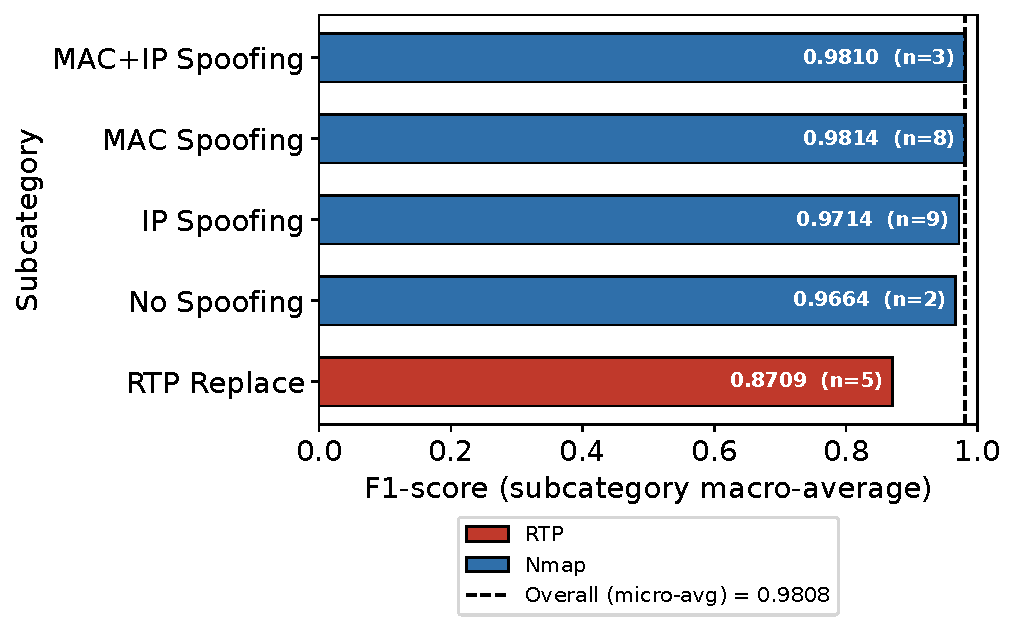
\includegraphics[width=\columnwidth]{figs/main_results_bars.pdf}
\caption{Detection F1 by attack subcategory (macro-average within subcategory) for the proposed method, ordered from hardest to easiest. Bar color indicates the parent category: RTP (red) vs.\ Nmap (blue); $n$ denotes the number of files in each subcategory. The dashed line marks the overall micro-average F1 across all 27 files (0.9808).}
\label{fig:main_bars}
\end{figure}

\noindent\textbf{Threshold-Independent Evaluation.}
To complement the fixed-threshold results above, we additionally report the area under the ROC curve (AUROC) and the area under the precision--recall curve (AUPRC), which characterize detection performance independently of the choice of $\tau$. Figures~\ref{fig:roc_pr}(a) and~\ref{fig:roc_pr}(b) show the ROC and precision--recall curves of the proposed method, aggregated by attack category. Table~\ref{tab:rocprc} summarizes the corresponding AUROC and AUPRC values.

\begin{figure}[pos=htbp]
\centering
\begin{subfigure}[b]{\columnwidth}
    \centering
    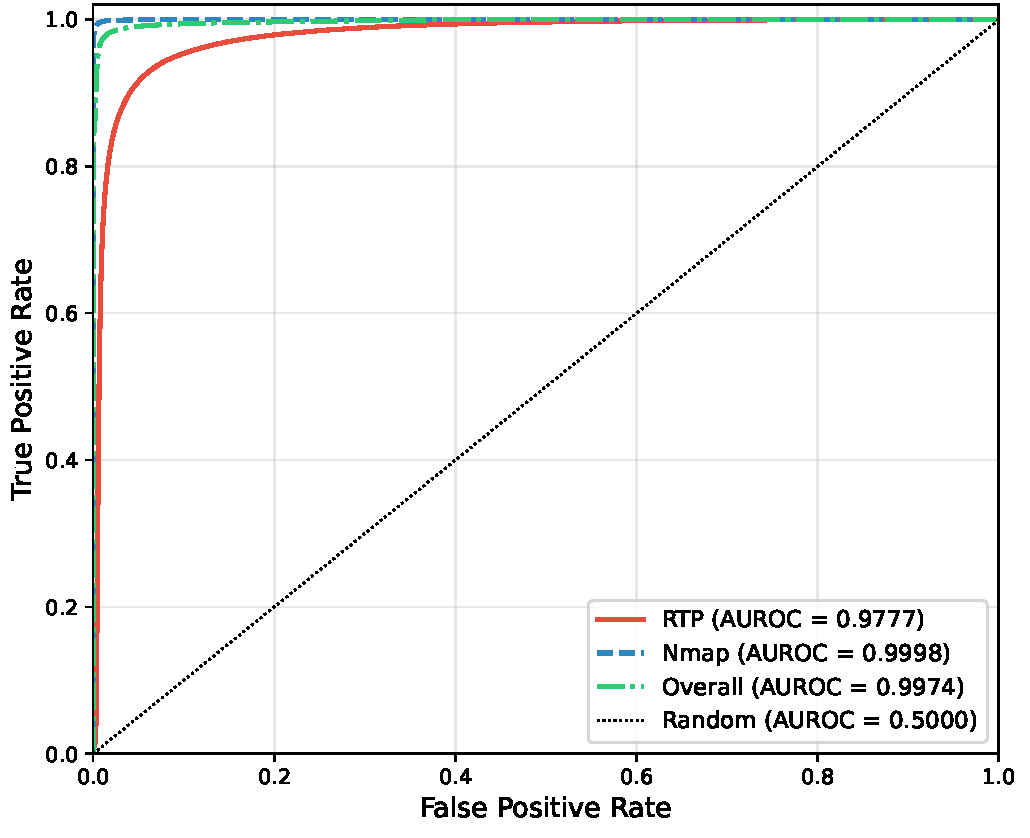
\includegraphics[width=\linewidth]{figs/roc_curve_proposed.pdf}
    \caption{ROC curves}
    \label{fig:roc}
\end{subfigure}

\vspace{2mm}

\begin{subfigure}[b]{\columnwidth}
    \centering
    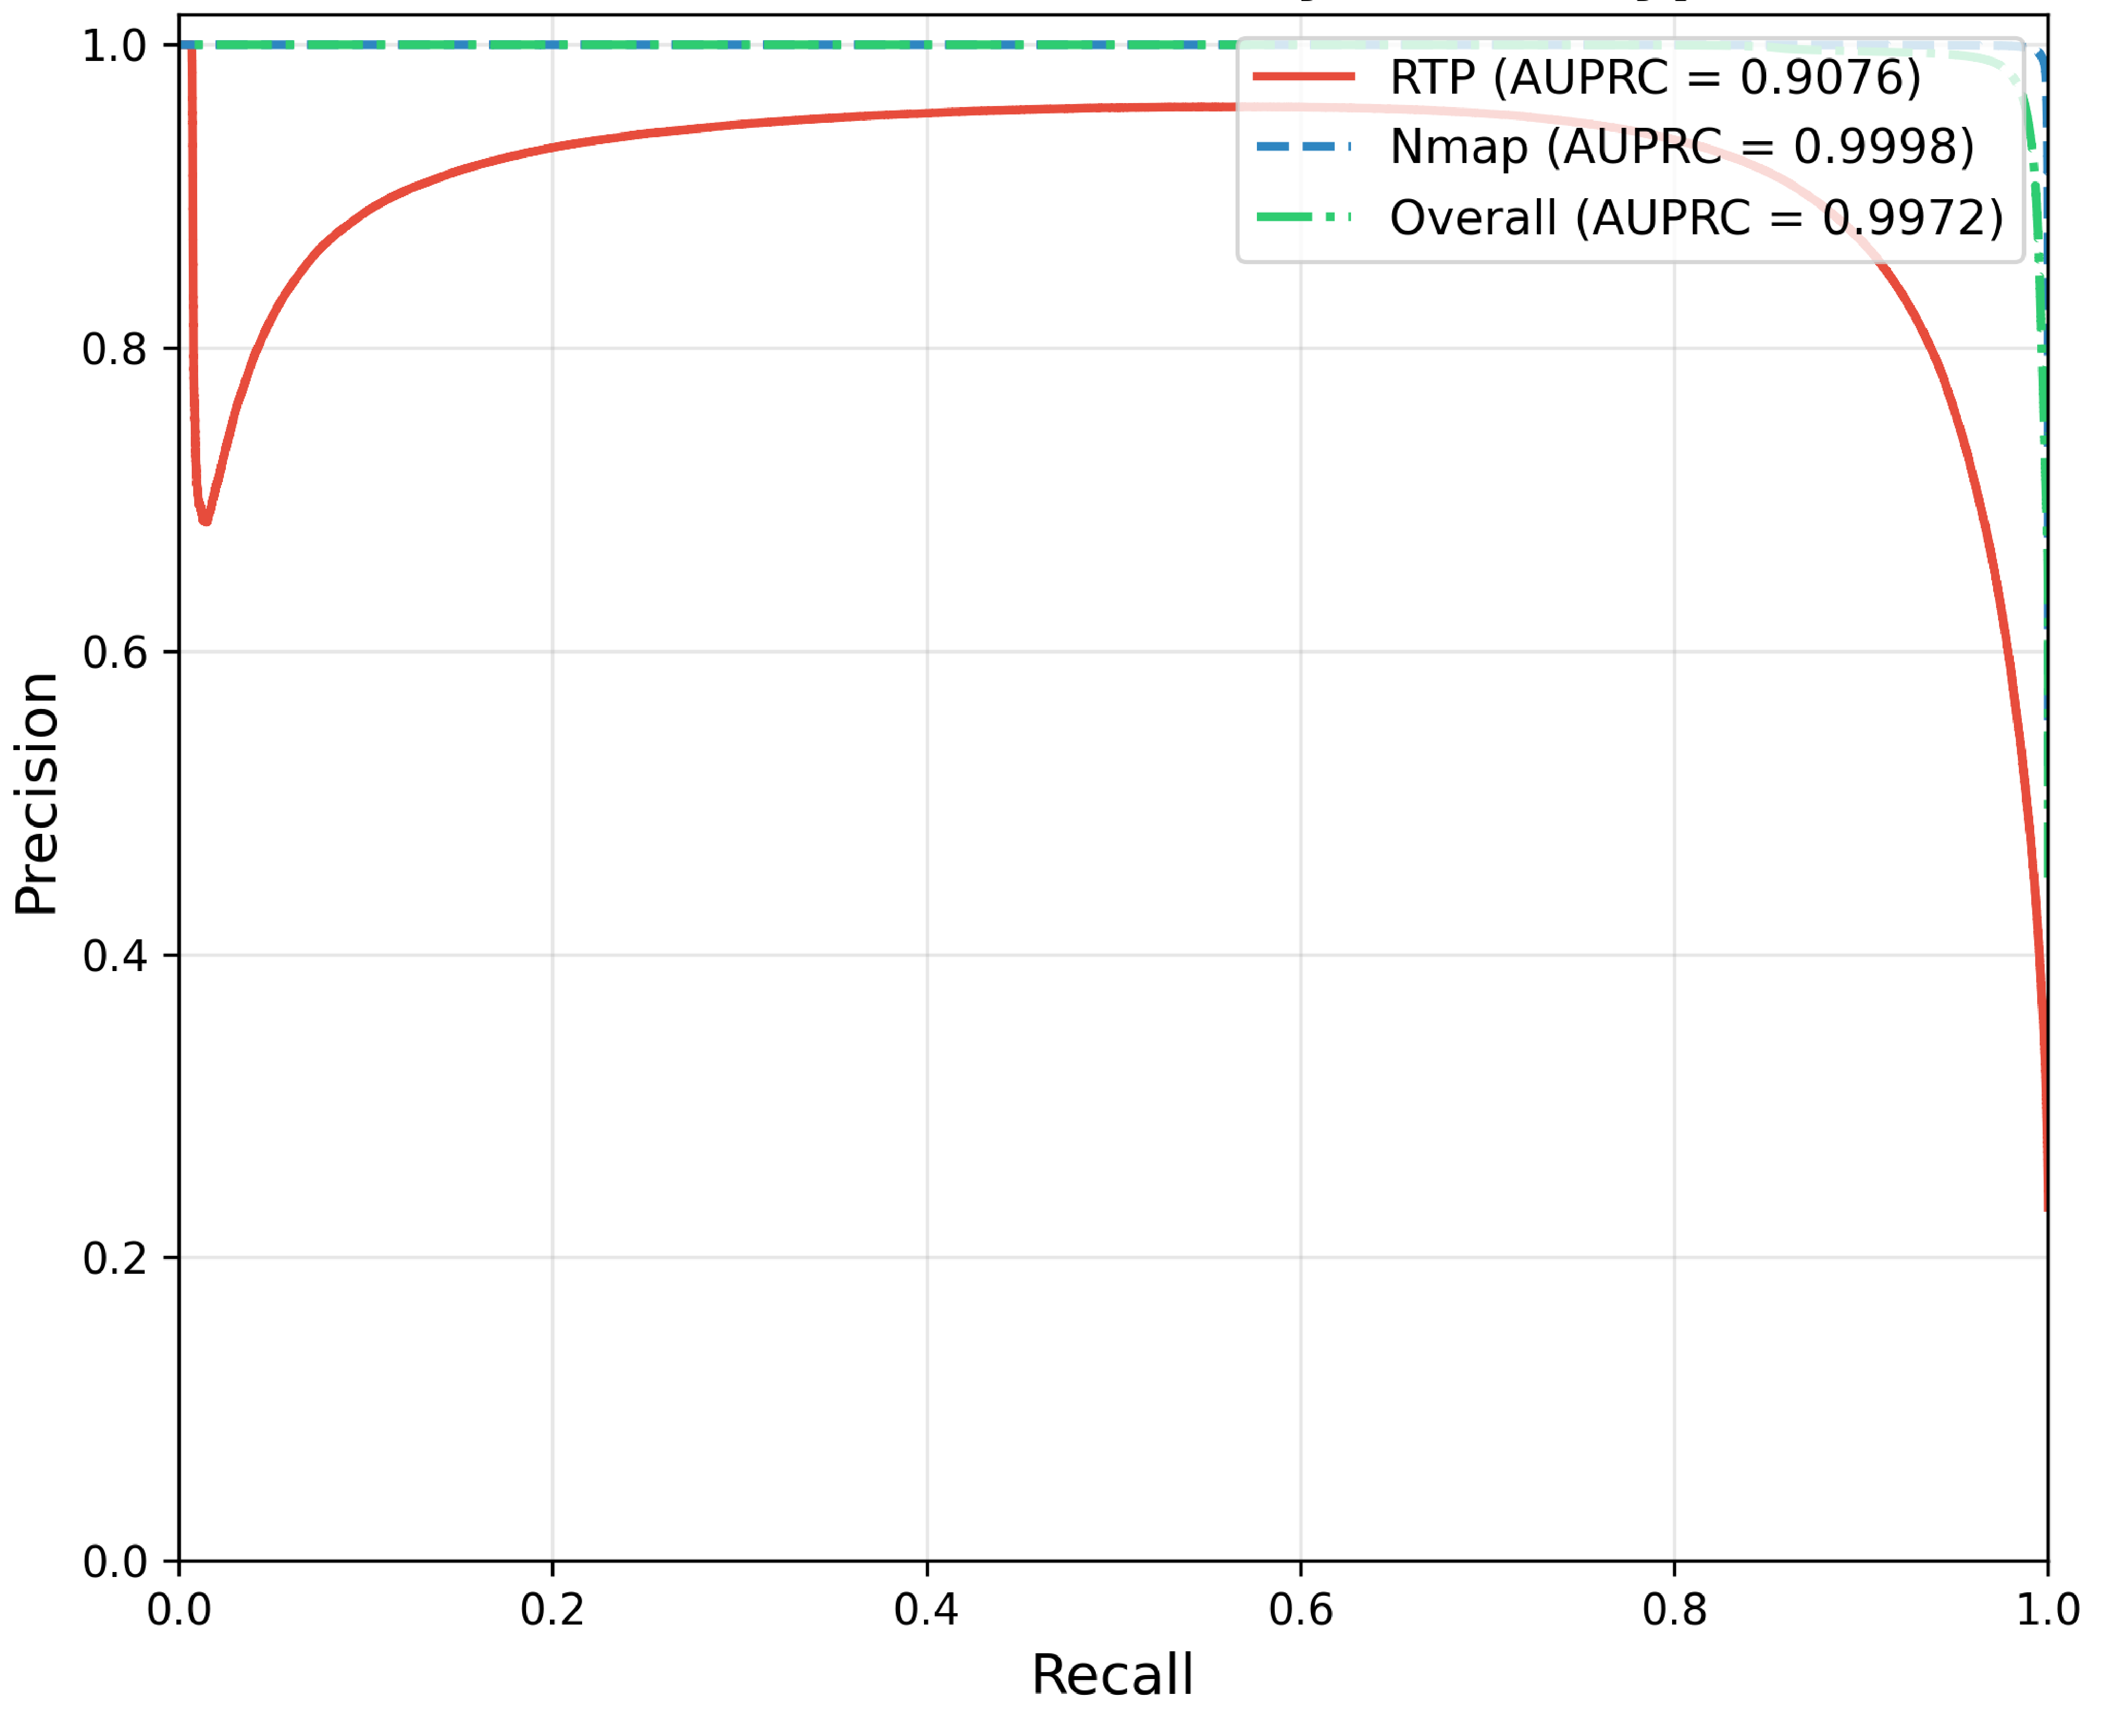
\includegraphics[width=\linewidth]{figs/pr_curve_proposed.pdf}
    \caption{Precision--recall curves}
    \label{fig:pr}
\end{subfigure}
\caption{ROC curves (a) and precision--recall curves (b) for the proposed method (Transformer-CNN with time-aware positional encoding). Each curve is computed by pooling all predictions within the corresponding attack category (micro-average within category).}
\label{fig:roc_pr}
\end{figure}

\begin{table}[!htbp]
\centering
\caption{AUROC and AUPRC for the proposed method (Transformer-CNN with time-aware positional encoding). Category rows: micro-avg within category; \textbf{Overall}: micro-avg across all 27 files.}
\label{tab:rocprc}
\footnotesize
\adjustbox{max width=\columnwidth}{%
\begin{tabular}{lcc}
\toprule
\textbf{Category} & \textbf{AUROC} & \textbf{AUPRC} \\
\midrule
RTP Stream Replacement     & 0.9777 & 0.9076 \\
Nmap Scanning \& Spoofing  & 0.9998 & 0.9998 \\
\midrule
\textbf{Overall (micro)}   & \textbf{0.9974} & \textbf{0.9972} \\
\bottomrule
\end{tabular}}
\end{table}

AUPRC is read against the class prevalence of each split, which is the score a no-skill detector would obtain (Table~\ref{tab:dataset}): 0.524 for the Nmap category, 0.233 for RTP, and 0.451 overall. Consistent with the fixed-threshold results, Nmap-based attacks achieve near-perfect AUROC and AUPRC (0.9998 each; Table~\ref{tab:rocprc}), reflecting a wide margin between normal and anomalous anomaly scores that is robust to the choice of $\tau$. RTP stream replacement attacks attain an AUROC of 0.9777 and an AUPRC of 0.9076 (Table~\ref{tab:rocprc}), indicating stronger separability than the fixed-threshold F1 results alone suggest; the anomaly scores consistently rank attack windows above normal ones, though the F1 gain at any single threshold remains bounded by the intrinsic difficulty of this attack category.

We note a localized dip in the pooled RTP precision--recall curve at low recall (Figure~\ref{fig:roc_pr}(b)), where precision briefly falls from 1.0 to approximately 0.70 before recovering to a plateau above 0.95. This pattern arises from heterogeneity across the five RTP files underlying the pooled curve: per-file AUPRC ranges from 0.8409 (SD-University-RearCamera-ReplaceRTP, the hardest file) to 0.9444 (RD-University-RearCamera-ReplaceRTP\_1, the easiest). The highest-ranked predictions at the most conservative operating points (lowest recall) are dominated by attack windows from the easiest file, for which the error margin from normal traffic is largest. As the threshold is lowered to admit predictions from harder files, a small number of normal windows are interleaved with true positives before recall increases far enough into the harder files' score distributions for precision to recover; this is a pooling artifact of combining five files with unequal detection difficulty into a single curve, rather than evidence of an unstable decision boundary. The subsequent decline at high recall (precision falls to approximately 0.4 as recall approaches 1.0) reflects the conventional PR curve tail effect: achieving recall on the single hardest-to-detect windows in the hardest file requires a threshold permissive enough to also admit a substantial number of normal windows.

\subsection{Comparison with Existing Methods}
\label{sec:baseline}
We compare the proposed method against three representative existing approaches for Automotive Ethernet intrusion detection, each re-implemented and evaluated on the same CarDS traces: (1) a supervised CNN-based detector originally proposed for replay-attack detection in AVTP streams~\cite{jeong2021convolutional}, published in this journal; (2) AERO, an unsupervised real-time anomaly observer for in-vehicle networks that relies on an engineered, protocol-informed feature extractor~\cite{jeong2023aero}; and (3) a feature-aware semi-supervised learning approach for Automotive Ethernet~\cite{shibly2023feature}. Two of these baselines cannot be run without supervision, and we therefore evaluate them under the assumption that labels are available: the CNN detector is given the full attack labels its training procedure requires, and the semi-supervised approach the labeled fraction it assumes. Both are trained and scored under five-fold cross-validation stratified by attack family, so that every family is represented in training while each attack capture is held out exactly once; the reported figures are the resulting out-of-fold predictions, and captures belonging to the same attack scenario are never split across a fold boundary. No supervised baseline is therefore scored on a capture it was trained on. AERO, like the proposed method, is trained on benign traffic only and uses the same benign split. The proposed method receives no attack labels at any stage. This comparison is consequently not label-matched, and the asymmetry runs \emph{against} the proposed method --- most strongly for the fully supervised CNN, and to a lesser degree for the semi-supervised classifier. We report it nonetheless, because the practically relevant question is how far a label-free detector falls short of methods that are granted the supervision they need; the CNN row is therefore best read as a label-privileged reference point rather than as a competing method under equal conditions. Because a supervised classifier, a per-capture-calibrated anomaly detector, and a reconstruction-based scorer do not share a common decision rule, each baseline is additionally evaluated at its own native operating point, and we adopt the threshold-independent AUROC as the primary basis for comparison, reporting F1 for reference only. Table~\ref{tab:baseline} summarizes the learning paradigm, feature representation, and detection performance of each baseline alongside the proposed method.


\begin{table*}[!tbp]
\centering
\caption{Comparison with prior Automotive Ethernet IDS on CarDS. AUROC is the primary, threshold-independent metric; per-row F1 is at each method's native operating point and not directly comparable. Bold marks the proposed method, not the column maximum. $\dagger$Approximate reproduction (no reference implementation); $\ddagger$Best AUROC over the AERO sweep.}
\label{tab:baseline}
\footnotesize
\begin{tabular}{lccccc}
\toprule
\textbf{Method} & \textbf{Paradigm (labels)} & \textbf{Feature} & \textbf{Params} & \textbf{AUROC} & \textbf{F1} \\
\midrule
CNN~\cite{jeong2021convolutional}   & Supervised (100\%)     & Protocol-specific (AVTP) & 1.36M & 0.999           & 0.995 \\
Semi-Sup.~\cite{shibly2023feature}  & Semi-supervised (10\%) & Feature-aware$^\dagger$  & --    & 0.96            & 0.88  \\
AERO~\cite{jeong2023aero}           & Unsupervised (0\%)     & Engineered (multimodal)  & 289k  & 0.81$^\ddagger$ & 0.32  \\
\midrule
Proposed                            & Self-supervised (0\%)  & Raw byte (agnostic)      & 898k  & \textbf{0.9974} & \textbf{0.9808} \\
\bottomrule
\end{tabular}
\end{table*}

\begin{table*}[!tbp]
\centering
\caption{Per-category detection AUROC on CarDS (threshold-independent, micro-avg within category); among the label-free methods, the proposed method alone remains strong on both categories. Bold marks the proposed method, not the column maximum. $\dagger$Approximate reproduction.}
\label{tab:baseline_perattack}
\footnotesize
\begin{tabular}{lcccc}
\toprule
\textbf{Attack category} & \textbf{CNN} & \textbf{Semi-Sup.$^\dagger$} & \textbf{AERO} & \textbf{Proposed} \\
                         & {\footnotesize sup.\ (100\%)} & {\footnotesize semi (10\%)} & {\footnotesize unsup.\ (0\%)} & {\footnotesize self (0\%)} \\
\midrule
RTP Stream Replacement    & 0.999 & 0.74--0.84 & 0.89       & \textbf{0.9777} \\
Nmap Scanning \& Spoofing & 0.997 & $\sim$1.00 & 0.50--0.76 & \textbf{0.9998} \\
\bottomrule
\end{tabular}
\end{table*}

On the threshold-independent AUROC, which is directly comparable across the differing operating points, the proposed method (0.9974) essentially matches the fully supervised CNN detector (0.999) despite using no attack labels, and exceeds both the semi-supervised (0.96) and the unsupervised AERO (0.81) baselines. The comparison with AERO---the only other label-free method, and thus the most directly comparable prior art---is the central result: 0.9974 versus 0.81. We prioritize AUROC over F1 because the three baselines occupy incompatible operating regimes: the supervised CNN emits near-binary sigmoid scores, AERO is calibrated per capture, and both degrade sharply if forced onto the single global percentile threshold used by the proposed reconstruction score. A per-category breakdown (Table~\ref{tab:baseline_perattack}) further reveals that the two prior detectors fail on \emph{complementary} attack categories: AERO collapses to near-random on Emergency/VLAN\,4 Nmap scans (AUROC 0.50), whereas the semi-supervised classifier---strong on scans owing to its partial labels---is weakest on RTP stream replacement (AUROC 0.74--0.84). The proposed method is the only label-free approach that remains strong on both categories (RTP 0.978, Nmap 0.9998).

The proposed method is therefore, to our knowledge, the only approach in this comparison that requires neither labeled attack data nor protocol-specific feature engineering. Section~\ref{sec:baseline_discussion} takes up what that combination buys in a multi-protocol setting.

\subsection{Ablation Study}
\label{sec:ablation}
The ablation study validates four design axes in sequence. We first fix the positional encoding to the conventional sinusoidal scheme ($\mathbf{P}_{\text{enc}} = \mathbf{P}$ in Eq.~\ref{eq:posenc}) and compare stream architectures to identify the optimal backbone, Transformer-CNN (Section~\ref{sec:arch_ablation}). We then fix this backbone and compare the sinusoidal encoding against the proposed time-aware positional encoding (Eq.~\ref{eq:timepe}) to finalize the proposed method (Section~\ref{sec:pe_ablation}). Third, using the finalized proposed method (Transformer-CNN with time-aware PE), we verify that the adopted input byte length (128 bytes) remains optimal (Section~\ref{sec:bytelen_ablation}). Finally, we augment the proposed method with tshark-parsed RTP header fields to probe a protocol-dependent upper bound on detection performance (Section~\ref{sec:rtpheader_ablation}).

\subsubsection{Stream Architecture}
\label{sec:arch_ablation}
Table~\ref{tab:ablation_arch} compares four stream architecture configurations at the $P_{97}$ threshold, all using sinusoidal positional encoding for the content stream. \textbf{Content-only} uses only the Transformer stream on raw byte content without the delta stream. \textbf{CNN-CNN} replaces the Transformer stream with a second residual CNN encoder applied to the content input. \textbf{Transformer-Transformer} replaces the CNN stream with a second Transformer encoder applied to the delta input. \textbf{Transformer-CNN (backbone)} is the dual-stream architecture validated in this section, which is combined with the proposed time-aware positional encoding in Section~\ref{sec:pe_ablation} to form the final proposed method.

\begin{table}[!htbp]
\centering
\caption{Ablation study: stream architecture variants (threshold: $P_{97}$ for all, sinusoidal PE). Overall F1: micro-avg (all 27 files); RTP/Nmap F1: macro-avg within category.}
\label{tab:ablation_arch}
\small
\adjustbox{max width=\columnwidth}{%
\begin{tabular}{lccc}
\toprule
\multirow{2}{*}{\textbf{Variant}} & \multicolumn{3}{c}{\textbf{F1-score}} \\
\cmidrule(l){2-4}
 & Overall & RTP & Nmap \\
\midrule
Content-only                          & 0.9189 & 0.0384 & 0.9222 \\
CNN-CNN                                & 0.9425 & 0.4597 & 0.9474 \\
Trans-Trans                            & 0.9593 & 0.7273 & 0.9560 \\
Trans-CNN (backbone) & \textbf{0.9713} & \textbf{0.7983} & \textbf{0.9570} \\
\bottomrule
\end{tabular}}
\end{table}

The category-level breakdown reveals that architecture choices affect the two attack types differently (Table~\ref{tab:ablation_arch}). The content-only variant achieves an overall F1 of 0.9189 but an RTP F1 of only 0.0384, indicating that without the delta stream the model is essentially unable to detect RTP stream replacement. Its Nmap F1 (0.9222) remains competitive, suggesting that raw byte content alone provides sufficient discriminative signal for scanning and spoofing detection. The dual-stream variants substantially improve RTP detection: CNN-CNN (RTP F1 = 0.4597) and Transformer-Transformer (RTP F1 = 0.7273) both represent large gains over content-only, while Transformer-CNN achieves the highest RTP F1 of 0.7983 among protocol-agnostic configurations. Nmap F1 is similar across all dual-stream variants (0.9474--0.9570), indicating that the architecture choice has limited impact on scanning detection once a delta stream is present.

\subsubsection{Positional Encoding: Sinusoidal vs.\ Time-Aware}
\label{sec:pe_ablation}
Having established Transformer-CNN as the optimal backbone (Section~\ref{sec:arch_ablation}), this section fixes the architecture and varies only the positional encoding scheme. We compare (i) the sinusoidal positional encoding ($\mathbf{P}_{\text{enc}} = \mathbf{P}$ in Eq.~\ref{eq:posenc}) used as the fixed baseline in Section~\ref{sec:arch_ablation} against (ii) the proposed time-aware positional encoding (Eq.~\ref{eq:timepe}). Both variants share the identical Transformer-CNN backbone; the only difference is that the time-aware scheme conditions the content stream's positional signal on the IPI recorded at capture time, rather than on packet rank.

Because the two encoding schemes induce different reconstruction-error distributions on normal traffic, their respective optimal thresholds differ (sinusoidal: $P_{97}$; time-aware: $P_{99}$); we therefore compare both variants at their own empirically selected operating points. Table~\ref{tab:ablation_pe} reports this comparison.

\begin{table}[!htbp]
\centering
\caption{Ablation study: Comparing the conventional sinusoidal positional encoding (baseline) against the proposed time-aware positional encoding, on the fixed Transformer-CNN backbone. Each variant is read at its own best-overall-F1 threshold, selected on the evaluation files, so these are per-variant optima rather than unbiased estimates (Table~\ref{tab:ablation_pe_cat} is threshold-independent). Overall F1: micro-avg (all 27 files); RTP/Nmap F1: macro-avg within category.}
\label{tab:ablation_pe}
\small
\adjustbox{max width=\columnwidth}{%
\begin{tabular}{lcccc}
\toprule
\multirow{2}{*}{\textbf{Variant}} & \multirow{2}{*}{\textbf{Threshold}} & \multicolumn{3}{c}{\textbf{F1-score}} \\
\cmidrule(l){3-5}
 & & Overall & RTP & Nmap \\
\midrule
Sinusoidal (baseline) & $P_{97}$ & 0.9713 & 0.7983 & 0.9570 \\
Time-aware (proposed) & $P_{99}$ & \textbf{0.9808} & \textbf{0.8709} & \textbf{0.9759} \\
\bottomrule
\end{tabular}}
\end{table}

At their respective best operating points, time-aware encoding improves overall F1 from 0.9713 to 0.9808 ($+0.0095$), RTP F1 from 0.7983 to 0.8709 ($+0.0726$), and Nmap F1 from 0.9570 to 0.9759 ($+0.0189$; Table~\ref{tab:ablation_pe}). Because each variant is read at its own empirically selected threshold, these F1 differences are per-variant optima rather than unbiased estimates, and we therefore treat the threshold-independent comparison in Table~\ref{tab:ablation_pe_cat} --- which is unaffected by threshold selection --- as the primary evidence for the encoding change; it shows the same ordering, with RTP AUPRC rising from 0.8675 to 0.9076. The improvement is most pronounced for the RTP category under both views, suggesting that the benefit of time-aware positional conditioning is concentrated on RTP stream replacement detection. From a deployment perspective, a practically important advantage of the time-aware scheme is its threshold robustness: as shown in Section~\ref{sec:threshold}, the sinusoidal model's performance collapses sharply beyond $P_{97}$, whereas the time-aware model remains stable through $P_{99}$, offering a substantially wider usable operating range.

Table~\ref{tab:ablation_pe_cat} further breaks this comparison down by attack category using threshold-independent metrics (AUROC/AUPRC), which are unaffected by the differing threshold scales of the two variants and therefore provide the cleanest evidence of the underlying representational improvement.

\begin{table}[!htbp]
\centering
\caption{AUROC/AUPRC comparison between the conventional sinusoidal positional encoding (baseline) and the proposed time-aware positional encoding (threshold-independent). Category rows: micro-avg within category; Overall: micro-avg across all 27 files.}
\label{tab:ablation_pe_cat}
\small
\adjustbox{max width=\columnwidth}{%
\begin{tabular}{lcccc}
\toprule
\multirow{2}{*}{\textbf{Category}} & \multicolumn{2}{c}{\textbf{Sinusoidal (baseline)}} & \multicolumn{2}{c}{\textbf{Time-aware (proposed)}} \\
\cmidrule(lr){2-3}\cmidrule(l){4-5}
 & AUROC & AUPRC & AUROC & AUPRC \\
\midrule
RTP             & 0.9721 & 0.8675 & \textbf{0.9777} & \textbf{0.9076} \\
Nmap            & 0.9998 & 0.9998 & 0.9998 & 0.9998 \\
\midrule
\textbf{Overall (micro)} & 0.9973 & 0.9968 & \textbf{0.9974} & \textbf{0.9972} \\
\bottomrule
\end{tabular}}
\end{table}

Nmap detection is already near-saturated under sinusoidal encoding (AUROC/AUPRC $\approx 0.9998$) and remains unchanged with time-aware encoding, indicating that byte-level scanning and spoofing signatures are already well captured by the content and delta streams without timing information. RTP stream replacement, in contrast, shows a clear improvement in threshold-independent metrics: AUPRC increases from 0.8675 to 0.9076 ($+0.0401$), a substantially larger gain than the corresponding AUROC improvement ($+0.0056$), consistent with AUPRC's greater sensitivity to precision--recall tradeoffs under class imbalance. This gain is notable because RTP stream replacement does not itself perturb inter-packet timing (Section~\ref{sec:main_results}), yet the introduction of IPI-based positional conditioning improves separability. Possible mechanisms are discussed in Section~\ref{sec:discussion}.

\subsubsection{Input Byte Length}
\label{sec:bytelen_ablation}
Using the finalized proposed method (Transformer-CNN with time-aware positional encoding, Section~\ref{sec:pe_ablation}), we verify that the adopted 128-byte input length remains optimal. Table~\ref{tab:ablation_bytes} compares three input byte length configurations: 64, 128, and 256 bytes per packet.

\begin{table}[!htbp]
\centering
\caption{Ablation study: input byte length, evaluated on the proposed method (Transformer-CNN, time-aware PE). Each variant is read at its own best-overall-F1 threshold, selected on the evaluation files, so these are per-variant optima rather than unbiased estimates (Table~\ref{tab:ablation_pe_cat} is threshold-independent). Overall F1: micro-avg (all 27 files); RTP/Nmap F1: macro-avg within category.}
\label{tab:ablation_bytes}
\small
\adjustbox{max width=\columnwidth}{%
\begin{tabular}{lcccc}
\toprule
\multirow{2}{*}{\textbf{Byte Length ($L$)}} & \multirow{2}{*}{\textbf{Threshold}} & \multicolumn{3}{c}{\textbf{F1-score}} \\
\cmidrule(l){3-5}
 & & Overall & RTP & Nmap \\
\midrule
64 bytes             & $P_{99.9}$ & 0.9267 & 0.0154 & 0.9803 \\
128 bytes (adopted)  & $P_{99}$   & \textbf{0.9808} & \textbf{0.8709} & 0.9759 \\
256 bytes            & $P_{95}$   & 0.1697 & 0.5662 & 0.0683 \\
\bottomrule
\end{tabular}}
\end{table}

The category-level breakdown reveals that byte length affects the two attack types in opposite directions (Table~\ref{tab:ablation_bytes}). The 64-byte configuration achieves an overall F1 of 0.9267 and a high Nmap F1 of 0.9803, but only at the most conservative threshold in the sweep ($P_{99.9}$, $\tau=0.000349$), where so little traffic is flagged that RTP detection collapses to an F1 of 0.0154; the configuration is retained as usable only by the Nmap category, which dominates the window count. Combined Ethernet, IP, UDP, and RTP headers occupy approximately 54 bytes, leaving roughly 10 bytes of RTP payload at a 64-byte truncation point. More fundamentally, the mean reconstruction error on normal traffic at 64 bytes is itself close to zero ($\text{mean}=3\times10^{-6}$), so the error increase induced by RTP stream replacement is indistinguishable from this noise floor regardless of the chosen threshold. The 256-byte configuration shows the opposite failure: RTP F1 remains moderate at 0.5662, but Nmap F1 collapses to 0.0683. In the CarDS dataset, many packets are shorter than 256 bytes, producing extensive zero-padded regions that inflate the mean reconstruction error on normal traffic by more than $21\times$ relative to 128 bytes (mean: 0.007536 vs.\ 0.000351). The resulting best-available threshold ($\tau=0.022152$ at $P_{95}$) is over $22\times$ higher than for 128 bytes ($\tau=0.000995$ at $P_{99}$), pushing the majority of small-footprint Nmap packets below the detection threshold. The 128-byte configuration avoids both failure modes, capturing Ethernet, IP, and transport headers in full while minimizing zero-padding, and is retained as the default configuration.

\subsubsection{RTP Header Augmentation}
\label{sec:rtpheader_ablation}
Finally, to examine how much additional performance is attainable in deployment scenarios that do not require full protocol-agnosticism, we augment the final proposed method (Transformer-CNN with time-aware PE) with RTP header fields extracted via tshark~\cite{tshark}, processed as an additional encoding stream. This variant depends on explicit protocol parsing and is therefore limited in applicability to RTP-carrying segments, departing from the protocol-agnostic design goal central to this work. It thus serves only as a protocol-dependent upper bound, not as a candidate for the proposed method.

\begin{table}[!htbp]
\centering
\caption{The proposed method with and without RTP header augmentation. Each variant is read at its own best-overall-F1 threshold across the full sweep, selected on the evaluation files, so these are per-variant optima rather than unbiased estimates (Table~\ref{tab:ablation_pe_cat} is threshold-independent). Overall F1: micro-avg (all 27 files); RTP/Nmap F1: macro-avg within category.}
\label{tab:ablation_rtpheader}
\small
\adjustbox{max width=\columnwidth}{%
\begin{tabular}{lcccc}
\toprule
\multirow{2}{*}{\textbf{Variant}} & \multirow{2}{*}{\textbf{Threshold}} & \multicolumn{3}{c}{\textbf{F1-score}} \\
\cmidrule(l){3-5}
 & & Overall & RTP & Nmap \\
\midrule
Proposed method                & $P_{99}$ & 0.9808 & 0.8709 & \textbf{0.9759} \\
+ RTP Header (upper bound)      & $P_{99}$ & \textbf{0.9882} & \textbf{0.9383} & 0.9688 \\
\bottomrule
\end{tabular}}
\end{table}

The RTP-header-augmented model improves overall F1 from 0.9808 to 0.9882 ($+0.0074$) at its best operating point, with the improvement concentrated on RTP stream replacement detection (RTP F1: 0.8709 $\rightarrow$ 0.9383, $+0.0674$; Table~\ref{tab:ablation_rtpheader}). Nmap detection, in contrast, regresses slightly (0.9759 $\rightarrow$ 0.9688, $-0.0071$), so the augmentation is not uniformly beneficial across categories. The RTP gain is expected, as explicit RTP header features directly encode per-packet sequence numbers and payload type identifiers that are highly discriminative for stream replacement detection. However, this variant requires tshark-based protocol parsing, limiting its applicability to RTP-carrying network segments in practice. The fully protocol-agnostic proposed method trades a modest performance gap against this upper bound for the practical benefit of deployability across arbitrary protocol mixes. Figure~\ref{fig:ablation_bars} visualizes this full progression, from the weakest architecture (content-only) through the finalized proposed method to its protocol-dependent upper bound.

\begin{figure}[pos=htbp]
\centering
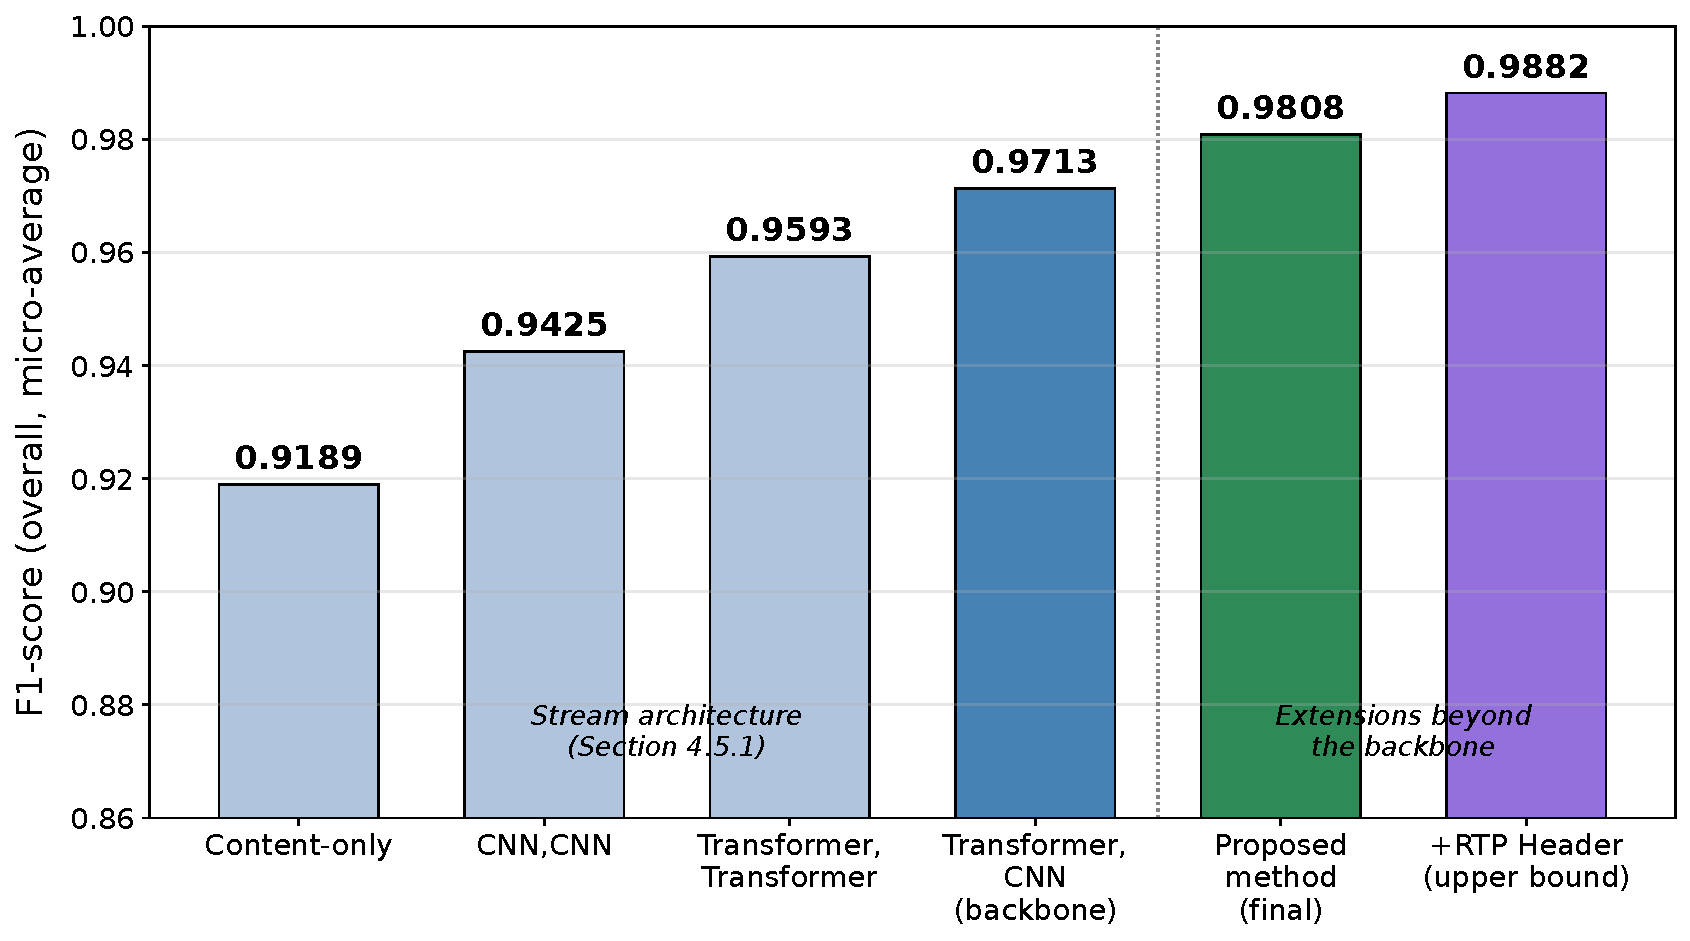
\includegraphics[width=\columnwidth]{figs/ablation_bars.pdf}
\caption{Overall micro-avg F1 across the ablation progression, from the weakest architecture (content-only) to the final proposed method and its protocol-dependent upper bound. Each configuration is evaluated at its own selected threshold, so bars are not directly comparable at a matched operating point (Section~\ref{sec:ablation}). Note the y-axis does not start at zero.}
\label{fig:ablation_bars}
\end{figure}

\subsection{Threshold Sensitivity}
\label{sec:threshold}
Table~\ref{tab:threshold} reports overall and RTP-category F1-scores across percentile thresholds for both positional encoding variants, illustrating how the precision--recall tradeoff shifts with threshold and motivating the selection of $P_{99}$ for the final proposed method.

\begin{table}[!htbp]
\centering
\caption{Threshold sensitivity, sinusoidal (baseline) vs.\ time-aware (proposed) positional encoding -- both on the fixed Transformer-CNN backbone -- evaluated at five percentile thresholds. Overall F1: micro-avg (all 27 files); RTP F1: macro-avg (5 RTP files).}
\label{tab:threshold}
\small
\adjustbox{max width=\columnwidth}{%
\begin{tabular}{lcccc}
\toprule
\multirow{2}{*}{\textbf{Threshold}} & \multicolumn{2}{c}{\textbf{Sinusoidal (baseline)}} & \multicolumn{2}{c}{\textbf{Time-aware (proposed)}} \\
\cmidrule(lr){2-3}\cmidrule(l){4-5}
 & Overall & RTP & Overall & RTP \\
\midrule
$P_{95}$   & 0.9641 & \textbf{0.8226} & 0.9521 & 0.7236 \\
$P_{97}$   & \textbf{0.9713} & 0.7983 & 0.9686 & 0.8052 \\
$P_{99}$   & 0.9277 & 0.1040 & \textbf{0.9808} & \textbf{0.8709} \\
$P_{99.5}$ & 0.9265 & 0.0738 & 0.9668 & 0.7224 \\
$P_{99.9}$ & 0.9225 & 0.0272 & 0.9219 & 0.0327 \\
\bottomrule
\end{tabular}}
\end{table}
Figure~\ref{fig:threshold} visualizes the data in Table~\ref{tab:threshold}. Both variants eventually collapse on RTP detection at sufficiently extreme thresholds ($P_{99.9}$), confirming that no fixed-threshold scheme is collapse-proof; the practically relevant difference is \emph{where this collapse begins relative to each model's own selected operating point}. The sinusoidal-PE model's RTP curve (red, dashed) collapses immediately beyond its selected threshold ($P_{97}$ $\rightarrow$ $P_{99}$), leaving no safety margin, whereas the time-aware model's RTP curve (green, dashed) rises to its maximum at its own selected threshold $P_{99}$ (0.8709), exceeding the best RTP F1 the sinusoidal variant reaches at any swept threshold (0.8226), and only begins declining one step past that point, at $P_{99.5}$. The selected operating point for each variant is marked with a star.

\begin{figure}[pos=htbp]
\centering
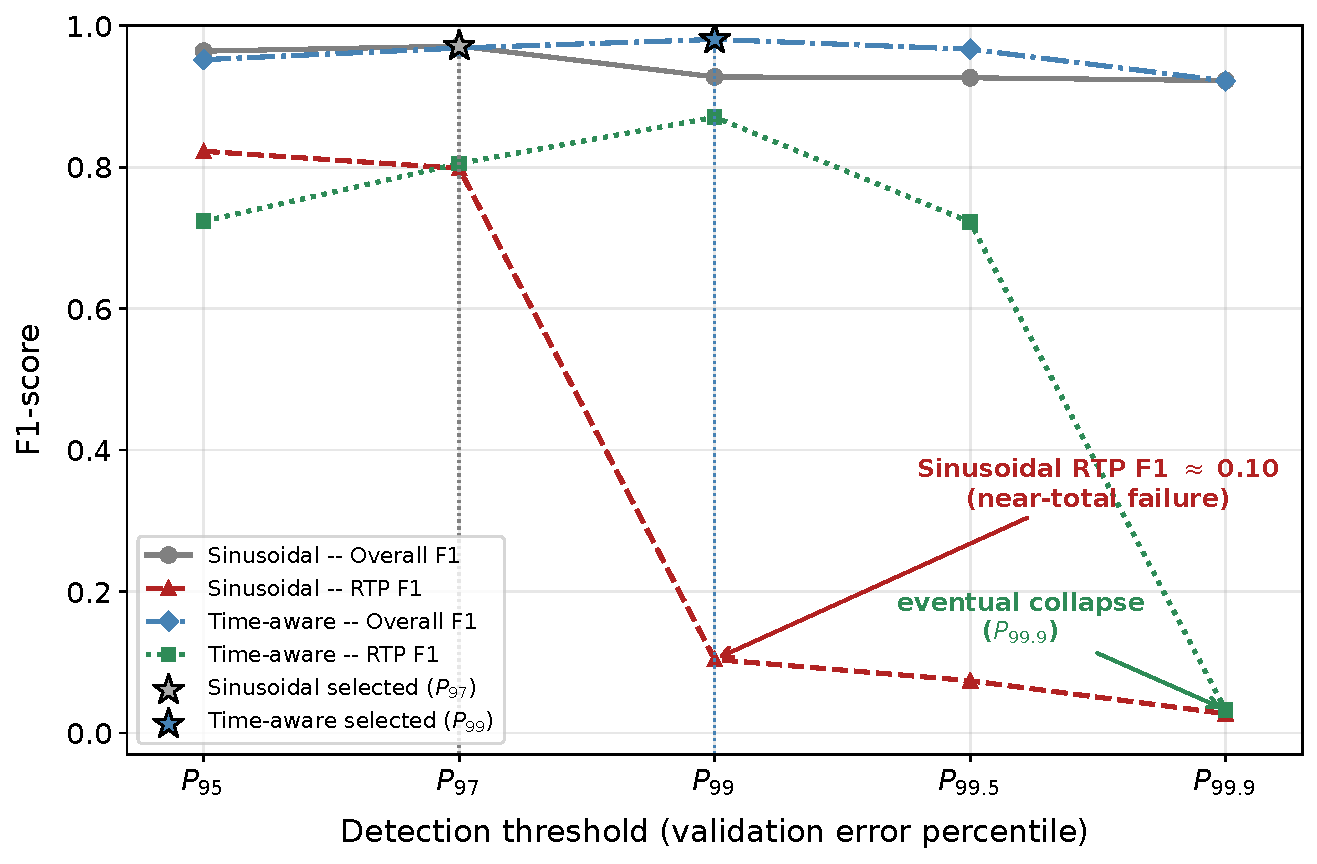
\includegraphics[width=\columnwidth]{figs/threshold_sensitivity.pdf}
\caption{F1-score as a function of detection threshold for the sinusoidal (baseline) and time-aware (proposed) positional encoding variants, shown for both the overall micro-average and the RTP stream replacement category. Stars mark each variant's selected operating threshold.}
\label{fig:threshold}
\end{figure}

The sinusoidal-PE model's overall F1 peaks at $P_{97}$ (0.9713) and then declines by $P_{99}$ (0.9277). This overall decline substantially understates the severity of the underlying failure: broken down by category, RTP stream replacement detection collapses almost completely, from an F1 of 0.7983 at $P_{97}$ to 0.1040 at $P_{99}$ and further to 0.0738 at $P_{99.5}$ and 0.0272 at $P_{99.9}$ -- a regime in which the model fails to detect the overwhelming majority of RTP attacks (average recall drops to approximately 6\% at $P_{99}$ and to roughly 1\% by $P_{99.9}$) while Nmap-based detection remains comparatively unaffected (average recall remains at approximately 98\% at $P_{99}$). This indicates that the sinusoidal model's usable operating range is narrow and asymmetric across attack categories: a threshold chosen based on overall F1 is liable to catastrophically fail on RTP-type attacks just one step higher in the swept grid, with no recovery at any of the higher percentiles evaluated.

The time-aware model exhibits qualitatively different behavior over the range relevant to deployment. Overall F1 continues to \emph{improve} through $P_{99}$ (0.9808, the global peak across all tested percentiles for either variant), with RTP F1 reaching 0.8709 -- exceeding the sinusoidal model's own peak RTP performance across all evaluated thresholds (0.8226, attained at $P_{95}$, one grid step before its selected operating threshold). Performance only begins to degrade one step past $P_{99}$, with a moderate decline at $P_{99.5}$ (RTP F1 = 0.7224) followed by a sharp collapse at $P_{99.9}$ (RTP F1 = 0.0327), reflecting a similarly complete functional collapse to the sinusoidal model's terminal value (0.0272) at the same percentile. This comparison clarifies the nature of the improvement: time-aware encoding does not render the model immune to threshold misspecification -- both variants ultimately fail at sufficiently extreme thresholds -- but it shifts the onset of severe collapse from the very next threshold step (sinusoidal: $P_{97}$ $\rightarrow$ $P_{99}$) to two steps beyond the selected threshold (time-aware: $P_{99}$ $\rightarrow$ $P_{99.9}$, with only a moderate decline at the intermediate $P_{99.5}$), providing a materially larger safety margin against threshold miscalibration in deployment. We select $P_{99}$ as the operating threshold for the final proposed method, as it coincides with the empirical peak of the overall F1-threshold curve in Table~\ref{tab:threshold} and is comfortably within the stable region rather than adjacent to the subsequent collapse observed at $P_{99.9}$.

Beyond motivating this choice, Table~\ref{tab:threshold} also lets us quantify the cost of label-free calibration (Section~\ref{sec:scoring}), in which $p$ is chosen to target a false-positive rate on unlabeled normal traffic alone rather than to maximize F1 on labeled attacks. Under label-free calibration, $p=95$ corresponds to a 5\% FPR. Relative to the labeled-calibration optimum at $P_{99}$ (Overall F1 = 0.9808, RTP F1 = 0.8709), label-free calibration at $P_{95}$ incurs a modest reduction in overall F1 (0.9808 $\rightarrow$ 0.9521, $-2.87$ points) but a substantially larger reduction in RTP-category F1 (0.8709 $\rightarrow$ 0.7236, $-14.73$ points, a relative decrease of approximately 16.9\%), consistent with the asymmetric sensitivity of the RTP category discussed above. Practitioners without access to labeled attacks should therefore expect reliable overall detection at $P_{95}$, with a meaningfully weaker margin specifically for stealthier attack categories such as RTP stream replacement.
\section{Discussion}
\label{sec:discussion}
\subsection{On the Baseline Comparison}
\label{sec:baseline_discussion}
Table~\ref{tab:baseline} (Section~\ref{sec:baseline}) situates the proposed method relative to three existing Automotive Ethernet IDS approaches spanning the full spectrum of label requirements, from fully supervised~\cite{jeong2021convolutional} to semi-supervised~\cite{shibly2023feature} to unsupervised~\cite{jeong2023aero}. Among these, AERO~\cite{jeong2023aero} is the most directly comparable in terms of label efficiency, as it is likewise trained without attack labels; the meaningful distinction is therefore not unsupervised learning per se, but \emph{what} the unsupervised model is trained on. AERO's feature extractor constructs three engineered, protocol-informed features prior to learning, whereas the proposed method operates directly on raw packet bytes. This distinction matters in a multi-domain, multi-protocol setting such as CarDS: a feature extractor tailored to one protocol's semantics (e.g., AVTP or SOME/IP) may require redesign when applied to a different protocol or network segment, whereas the proposed raw-byte representation generalizes across segments by construction. Quantitatively, this label-efficiency advantage manifests as a per-category complementarity in the baselines' failure modes: AERO, the only other label-free method, drops to near-random on Emergency/VLAN\,4 Nmap scans (AUROC 0.50) despite handling RTP replacement reasonably (0.89), whereas the semi-supervised classifier inverts this profile, remaining near-perfect on scans (AUROC $\approx$1.0) but weakest on RTP replacement (0.74--0.84). The proposed method attains strong detection on both categories (RTP 0.978, Nmap 0.9998) without any attack labels or protocol-specific features, which we attribute to a single raw-byte representation that generalizes across heterogeneous attack types where hand-crafted or partially labeled features do not.

\subsection{Analysis of RTP Stream Replacement Detection}
Of the two attack categories evaluated, RTP stream replacement presents a structurally distinct detection challenge because it preserves packet-level structure --- valid RTP headers, consistent inter-arrival timing, and comparable payload lengths --- while substituting only the video payload content. This narrows the reconstruction error margin between normal and anomalous traffic, which is reflected in the threshold-independent separability reported in Section~\ref{sec:main_results} (AUPRC 0.9076 vs.\ 0.9998 for Nmap-based attacks). The per-file variation in F1-score within the category (0.8265--0.9217) further suggests that detectability is partly governed by the statistical distance between the injected video content and the training distribution of normal camera traffic, independent of the attack mechanism itself. Attack files whose replacement content is statistically closer to the normal distribution present a harder detection target --- an inherent property of reconstruction-based anomaly detection that implies evasion difficulty varies with the attacker's choice of replacement payload.

A notable observation is that time-aware positional encoding (Section~\ref{sec:pe_ablation}) improves RTP detection by AUPRC $+0.0401$ despite RTP stream replacement deliberately \emph{preserving} inter-packet timing, implying the gain does not arise from direct detection of timing anomalies. We offer two non-exclusive hypotheses. First, conditioning the Transformer's self-attention on real IPI data may yield a more precise learned representation of normal traffic globally --- including aspects unrelated to timing irregularities --- such that the content stream becomes more discriminative for RTP payload reconstruction as a secondary benefit. Second, despite the attacker's intent to preserve timing, the frame-replacement mechanism may itself introduce subtle inter-arrival perturbations at the moment of stream substitution, which a model conditioned on raw timing data may be more sensitive to than a rank-only sinusoidal baseline. Distinguishing between these hypotheses would require attention-weight analysis or a controlled ablation that perturbs timing while holding payload content fixed; we leave this to future work.

\subsection{Practical Deployment Considerations}
The proposed method is designed with practical automotive deployment in mind. With time-aware positional encoding, the model comprises approximately 897.6K trainable parameters (excluding the protocol-aware RTP header stream evaluated in Section~\ref{sec:ablation}), an increase of fewer than 17K parameters ($<$2\%) over the sinusoidal-PE backbone (880.8K), since the IPI projection consists of only two small linear layers. This corresponds to a memory footprint of approximately 3.4\,MB in 32-bit precision, remaining well within the constraints of automotive-grade embedded hardware. Training is performed exclusively on normal traffic captured during vehicle operation, requiring no attack simulation or manual annotation.

A practical consideration in sliding-window inference is the latency introduced by the requirement to buffer $N = 64$ consecutive packets before issuing a detection decision. In the CarDS dataset, the average inter-packet interval on the evaluated network segments is on the order of microseconds to milliseconds, resulting in a window accumulation time of well under one second under normal traffic conditions. This latency is acceptable for most automotive intrusion detection use cases, in which near-real-time rather than hard-real-time detection is sufficient. Nevertheless, reducing the window size while maintaining detection performance remains an open direction for latency-sensitive deployments, and is left for future investigation.

\subsection{Limitations}
\label{sec:limitations}

The evaluation is drawn entirely from a single 2020 production EV, and although the attack set spans 23 configurations, these reduce to only two underlying mechanisms -- Nmap-based scanning/spoofing and RTP stream replacement -- leaving other attack classes (e.g., denial-of-service, firmware/OTA tampering, and the excluded REST API trace) untested. The 0.01\% exclusion threshold also means behavior against deliberately low-footprint, stealthy attackers -- arguably the most realistic adversary -- remains unverified. Broader validation across vehicles, topologies, and attack families is needed.

Sliding windows use stride 1, so consecutive windows share 63 of 64 packets. Precision, recall, and F1 treat each window as an independent sample, which is standard in window-based intrusion detection but does not hold strictly under this overlap; reported metrics are best read as characterizing detection over the continuous stream rather than over independent trials.

Threshold selection is the one point in the pipeline where labeled data is used. Each percentile candidate ($P_{95}$--$P_{99.9}$) is computed purely from the normal validation distribution; only the choice among candidates uses labeled attacks (Section~\ref{sec:scoring}), drawn from the same 27 files used for final reporting rather than a disjoint split. This dependency has limited practical consequence, for two related reasons. Table~\ref{tab:threshold} shows that overall and RTP F1 remain broadly stable from $P_{95}$ through $P_{99.5}$, and the threshold-independent AUROC (0.9974) and AUPRC (0.9972) confirm this reflects genuine separability rather than a favorable threshold pick, so nearly any reasonable choice in the swept range would have performed comparably; only the extreme $P_{99.9}$ collapses. This same stability is also what makes the threshold robust to deployment-time drift: validation-set thresholds are not guaranteed to transfer exactly to deployment traffic, since the reconstruction error distribution may shift due to vehicle aging, software updates, or driving conditions absent from training data, yet the sinusoidal-PE baseline's RTP detection collapses almost entirely with a single percentile shift beyond its optimum, whereas the time-aware model's stable region extends substantially further, giving a wider safety margin against such drift. Even so, a fully label-free calibration procedure, or a held-out calibration split disjoint from the test files, would close the labeling gap more rigorously.

A more fundamental limitation is that the method assumes packet content carries learnable structure. Under link-layer or transport-layer encryption (e.g., MACsec, IPsec), byte content becomes effectively high-entropy and reconstruction-based detection loses its signal, regardless of traffic class. Pervasive per-packet encryption remains uncommon in current in-vehicle networks, however, mirroring CAN's own long-standing lack of encryption under tight compute and real-time budgets. This makes the assumption reasonable for the segments evaluated here, but it is a boundary condition rather than a guarantee, and should be revisited as automotive encryption adoption evolves.
\section{Conclusion}
This paper presented an unsupervised dual-stream masked autoencoder for intrusion detection in Automotive Ethernet networks, addressing two fundamental challenges in automotive IDS development: protocol heterogeneity and the scarcity of annotated attack traffic. A sliding window of 64 consecutive packets is encoded through two complementary streams -- a Transformer encoder that captures global inter-packet dependencies from raw byte content, conditioned on a time-aware positional encoding derived from real inter-packet capture timing rather than fixed sequence rank, and a residual 1D-CNN encoder that models local per-byte temporal dynamics from inter-packet byte differences -- unified through a delta-conditioned gated residual fusion mechanism. The model is trained via packet-level masked reconstruction on unlabeled normal traffic alone, and anomalies are flagged at inference time by thresholding the mean reconstruction error against a percentile-based threshold derived from normal validation traffic.

Experiments on the CarDS Automotive Ethernet dataset, spanning 27 real-vehicle attack files across 23 attack configurations, show that the proposed method achieves an overall F1-score of 0.9808, AUROC of 0.9974, and AUPRC of 0.9972 at its selected operating threshold ($P_{99.9}$), essentially matching a fully supervised baseline (AUROC 0.999) while requiring no attack labels. Detection is near-perfect on Nmap-based scanning and spoofing attacks (F1 $>$ 0.95) but comparatively harder on RTP stream replacement (avg.\ F1 = 0.8709), which alters only payload content while preserving packet-level structure and timing. Ablation studies confirm that the dual-stream architecture and the time-aware positional encoding each contribute independently to detection performance, with the latter also substantially widening the range of thresholds over which performance remains stable.

Several limitations point to directions for future work. The method was evaluated on a single real-vehicle dataset covering two attack families (RTP stream replacement and Nmap-based scanning/spoofing); broader validation across vehicle platforms, network topologies, and attack types is needed to establish generalizability. Threshold calibration, the one place labeled attack data enters the pipeline, currently relies on a percentile search over labeled validation attacks, and less threshold-sensitive or fully label-free scoring schemes merit further study. The mechanism by which time-aware positional encoding improves RTP detection despite the attack itself preserving inter-packet timing also remains unclear and warrants attention-weight or controlled perturbation analysis. Finally, deploying the framework in online, resource-constrained settings -- including latency characterization and model compression for embedded ECU targets -- is an important direction for practical automotive IDS.

% Numbered list
% Use the style of numbering in square brackets.
% If nothing is used, default style will be taken.
%\begin{enumerate}[a)]
%\item 
%\item 
%\item 
%\end{enumerate}  

% Unnumbered list
%\begin{itemize}
%\item 
%\item 
%\item 
%\end{itemize}  

% Description list
%\begin{description}
%\item[]
%\item[] 
%\item[] 
%\end{description}  

% Uncomment and use as the case may be
%\begin{theorem} 
%\end{theorem}

% Uncomment and use as the case may be
%\begin{lemma} 
%\end{lemma}

%% The Appendices part is started with the command \appendix;
%% appendix sections are then done as normal sections
%% \appendix

% Renders the "CRediT authorship contribution statement" section from the
% \credit{} declarations attached to each author above.
\printcredits

\section*{Declaration of competing interest}
The authors declare that they have no known competing financial interests or personal
relationships that could have appeared to influence the work reported in this paper.

\section*{Data availability}
The CarDS Automotive Ethernet dataset analyzed in this study is publicly available and is
described by its authors in~\cite{hellemans2025cards}. No new data were generated in this study.

%% Loading bibliography style file
%\bibliographystyle{model1-num-names}
\bibliographystyle{cas-model2-names}

% Loading bibliography database
\bibliography{reference}

% Biography
\bio{}
\noindent\textbf{Yeonjae Kang} is a Ph.D. candidate at the School of Cybersecurity, Korea University, Seoul, Republic of Korea, where she is a member of the Hacking and Countermeasure Research Lab. Her research interests include in-vehicle network security, intrusion detection, and machine learning for security applications.
\endbio

\bio{}
\noindent\textbf{Huy Kang Kim} received the B.S., M.S., and Ph.D. degrees from the Korea Advanced Institute of Science and Technology (KAIST). He founded A3 Security Consulting, the first information security consulting company in South Korea, in 1999. He is currently a Professor with the School of Cybersecurity, Korea University, Seoul, Republic of Korea. His research interests include vehicle security, network security, and anomaly detection based on machine learning.
\endbio

\bio{}
\noindent\textbf{Seonghoon Jeong} received the Ph.D. degree from the School of Cybersecurity, Korea University, Seoul, Republic of Korea. He is currently an Assistant Professor with the Division of Artificial Intelligence Engineering, Sookmyung Women's University, Seoul, Republic of Korea. His research interests include in-vehicle network security, Automotive Ethernet, and intrusion detection systems.
\endbio

\end{document}

